
\subsection{シミュレーション実験の目的}
4.1章,4.2章のシミュレーション実験によって,
最小半径を140mmに設定することで,
脚軌道生成に失敗することなく直進動作,旋回動作を行えることが確認された.
そこで本章では,これらの直進動作と旋回動作を組み合わせた場合でも,
最小半径を140mmに設定することで,
脚軌道生成に失敗することなく歩行することができるか確認する.
これによって,最小半径を140mmに設定することが脚軌道生成の失敗を防ぐために有効であるかを検証することを目的とする.

本章では新たに実装した,自由歩容パターン生成手法を統合したプログラムを用いて,
直進動作と旋回動作を組み合わせた歩容パターンを生成し,
脚軌道生成に失敗することなく歩行できること,
また指定した通りに動作を切り替えることができることを確認する.

\subsection{シミュレーション実験の条件}
シミュレーションを行うソフトウェア,シミュレーションを行う計算環境,
モデルとするロボットは直進動作のシミュレーション実験と同様であるため説明を省略する.
歩行条件についても直進動作のシミュレーション実験および,
旋回動作のシミュレーション実験と同様とする.

\subsubsection{歩行する経路}
本シミュレーション実験で用いる,ロボットが歩行する経路は,
直進動作と旋回動作を含む歩容パターンを生成する必要があるような経路である必要となる.
そのような経路のうち,単純な経路として,
始点から1000mm直進したのち,$180^{\circ}$旋回を行って,再び1000mm直進させ始点に戻る経路をシミュレーションで用いた.

地形は平面,130mmの段差がある地形,15度傾斜した地形の3つの地形を用いる.
平面な地形を用いる場合の経路を\figref{fig:ch4_integration_flat_map}に示した.
また,130mmの段差がある地形を用いる場合の経路を\figref{fig:ch4_integration_130mm_map}に,
15度傾斜した地形を用いる場合の経路を\figref{fig:ch4_integration_15deg_map}に示した.
\figref{fig:ch4_integration_flat_map},
\figref{fig:ch4_integration_130mm_map},
\figref{fig:ch4_integration_15deg_map}では
ロボットが直進する方向にx軸,ロボット上向きにz軸とるようなワールド座標系を用いる.
平面な地形では,始点を$(0,0,0)$,中継点を$(1000,0,0)$,終点を$(0,0,0)$とする.
130mmの段差がある地形では,始点を$(0,0,0)$,中継点を$(1000,0,130)$,終点を$(0,0,0)$とする.
15度傾斜した地形では,始点を$(0,0,0)$,中継点を$(1000,0,129.5)$,終点を$(0,0,0)$とする.

\newpage

% chapter4/integration_flat_map.png
\begin{figure}[htbp]
  \begin{center}
    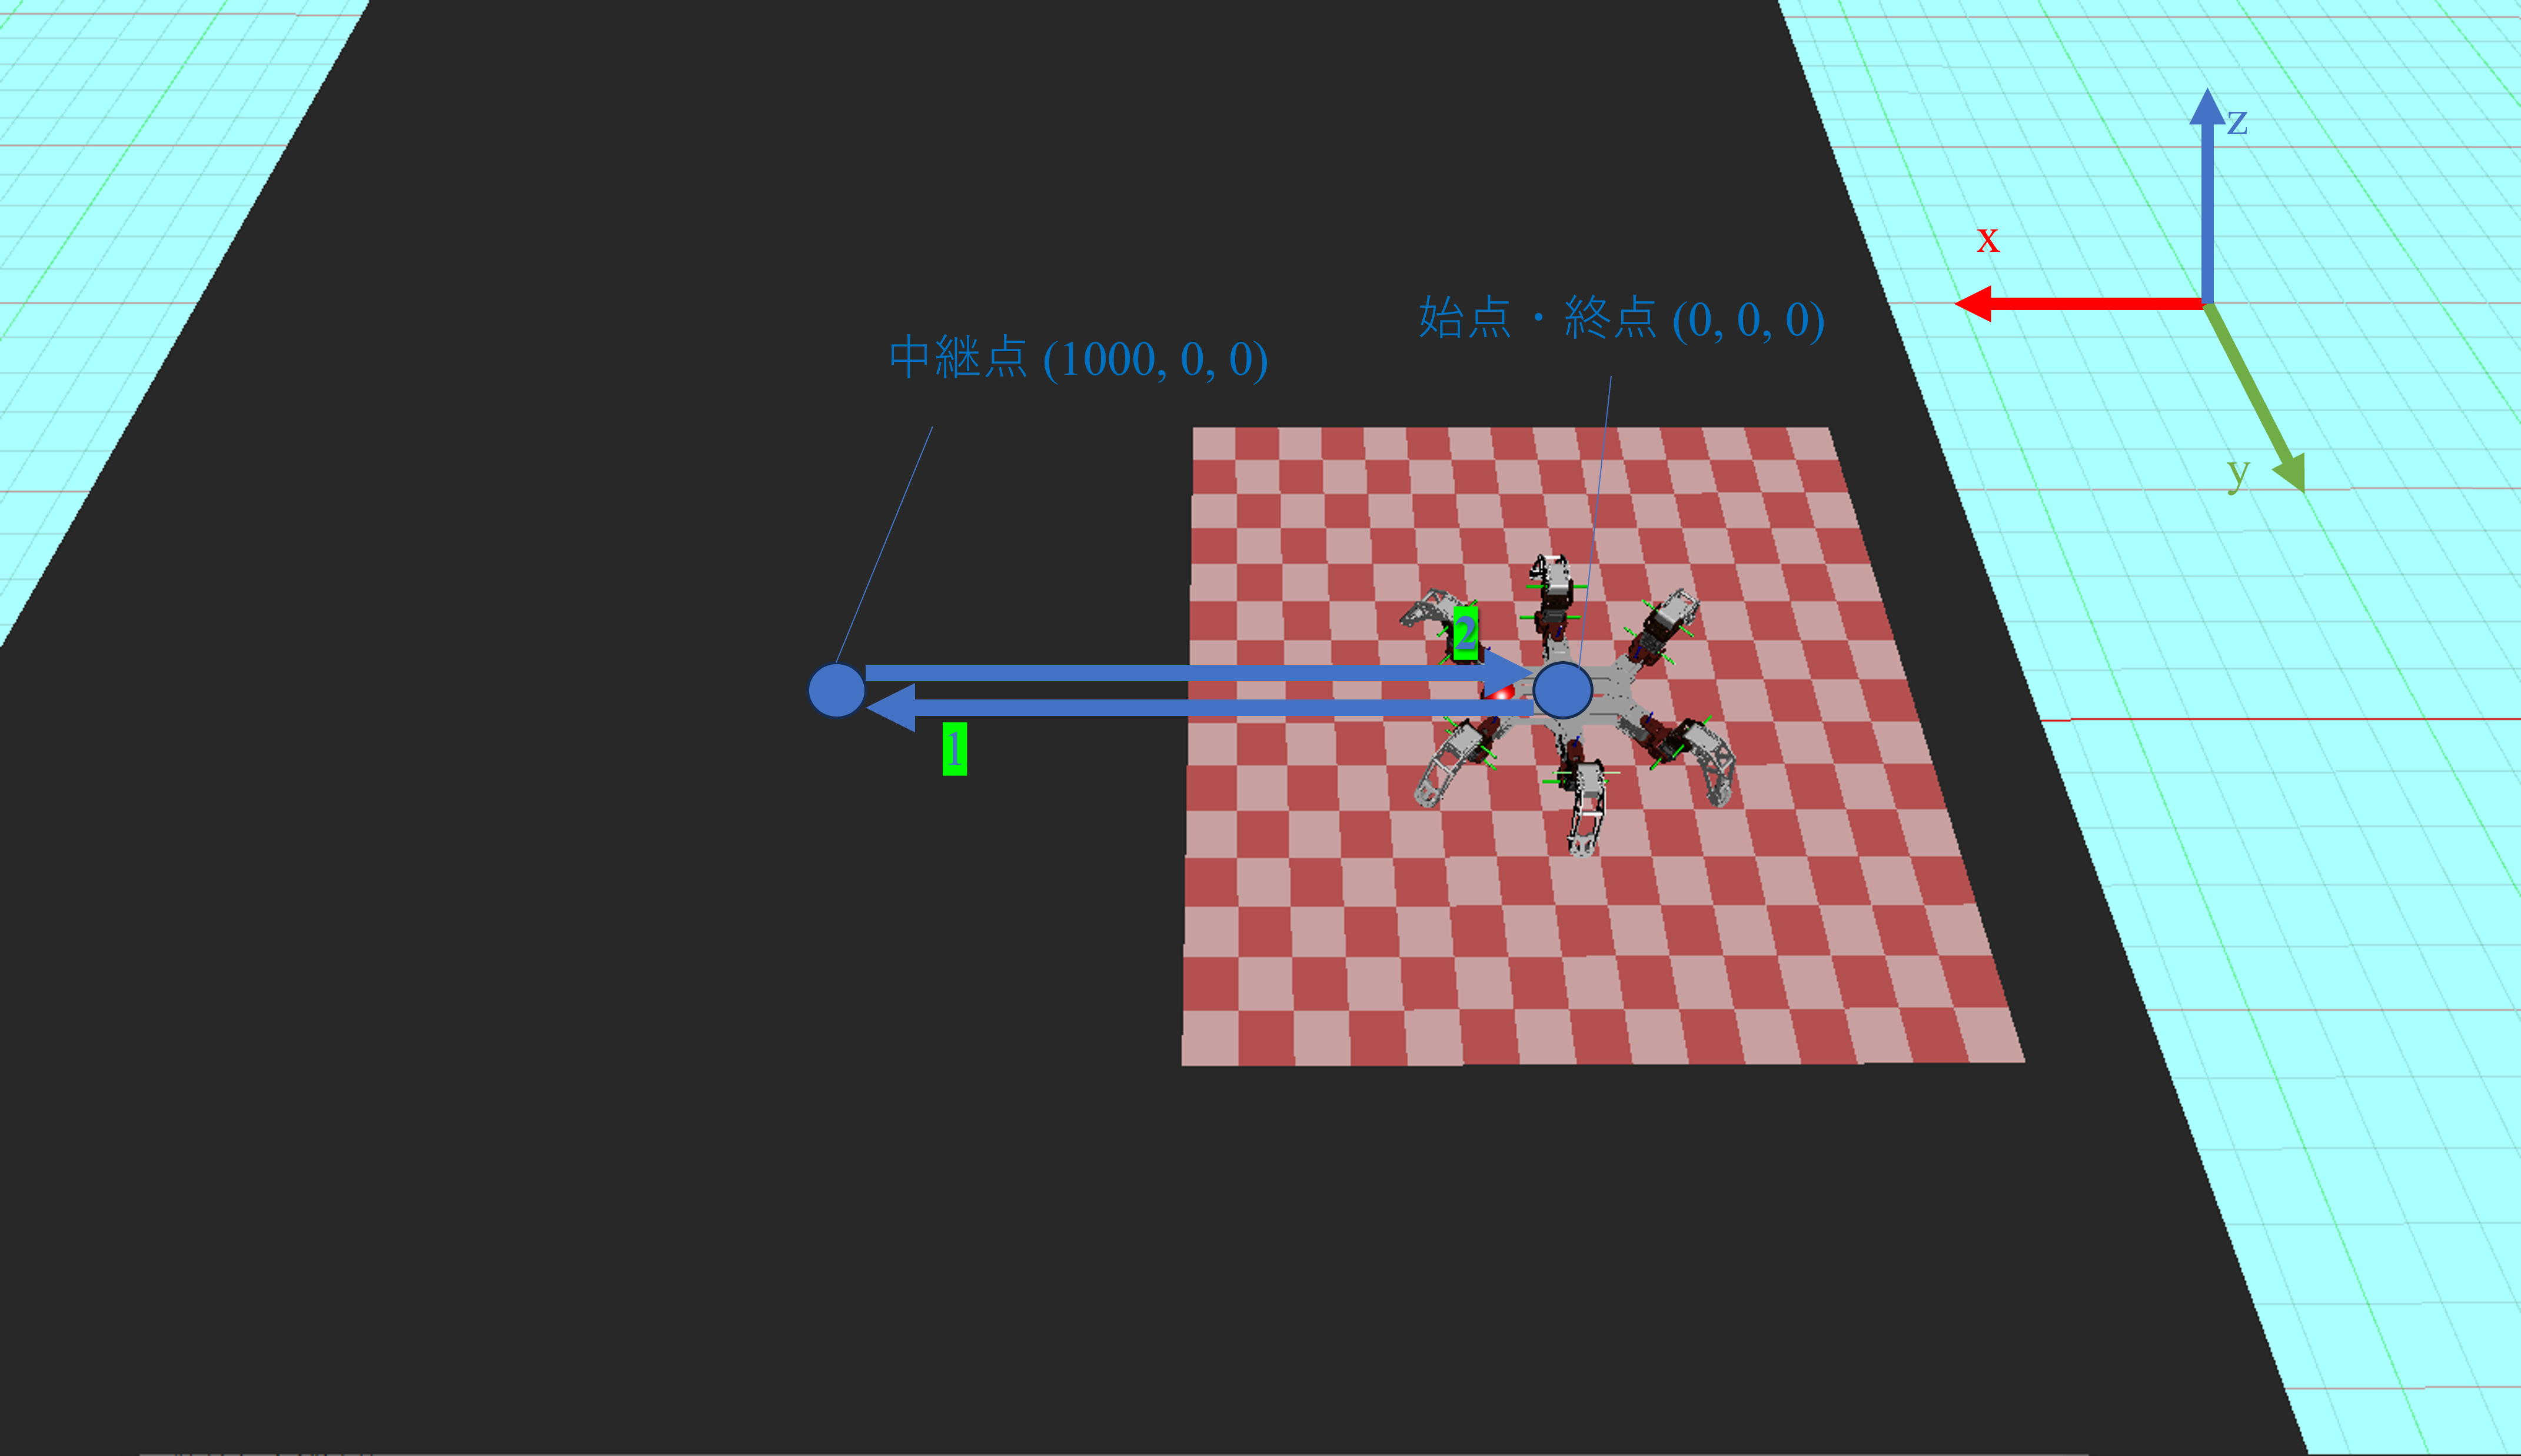
\includegraphics[width=0.7\linewidth,trim={0 50 0 0}, clip]{figure/chapter4/integration_flat_map.png}
    \caption{Route of Movement on Flat Terrain}
    \label{fig:ch4_integration_flat_map}  % chktex 24
  \end{center}
\end{figure}

% chapter4/integration_130mm_map.png
\begin{figure}[htbp]
  \begin{center}
    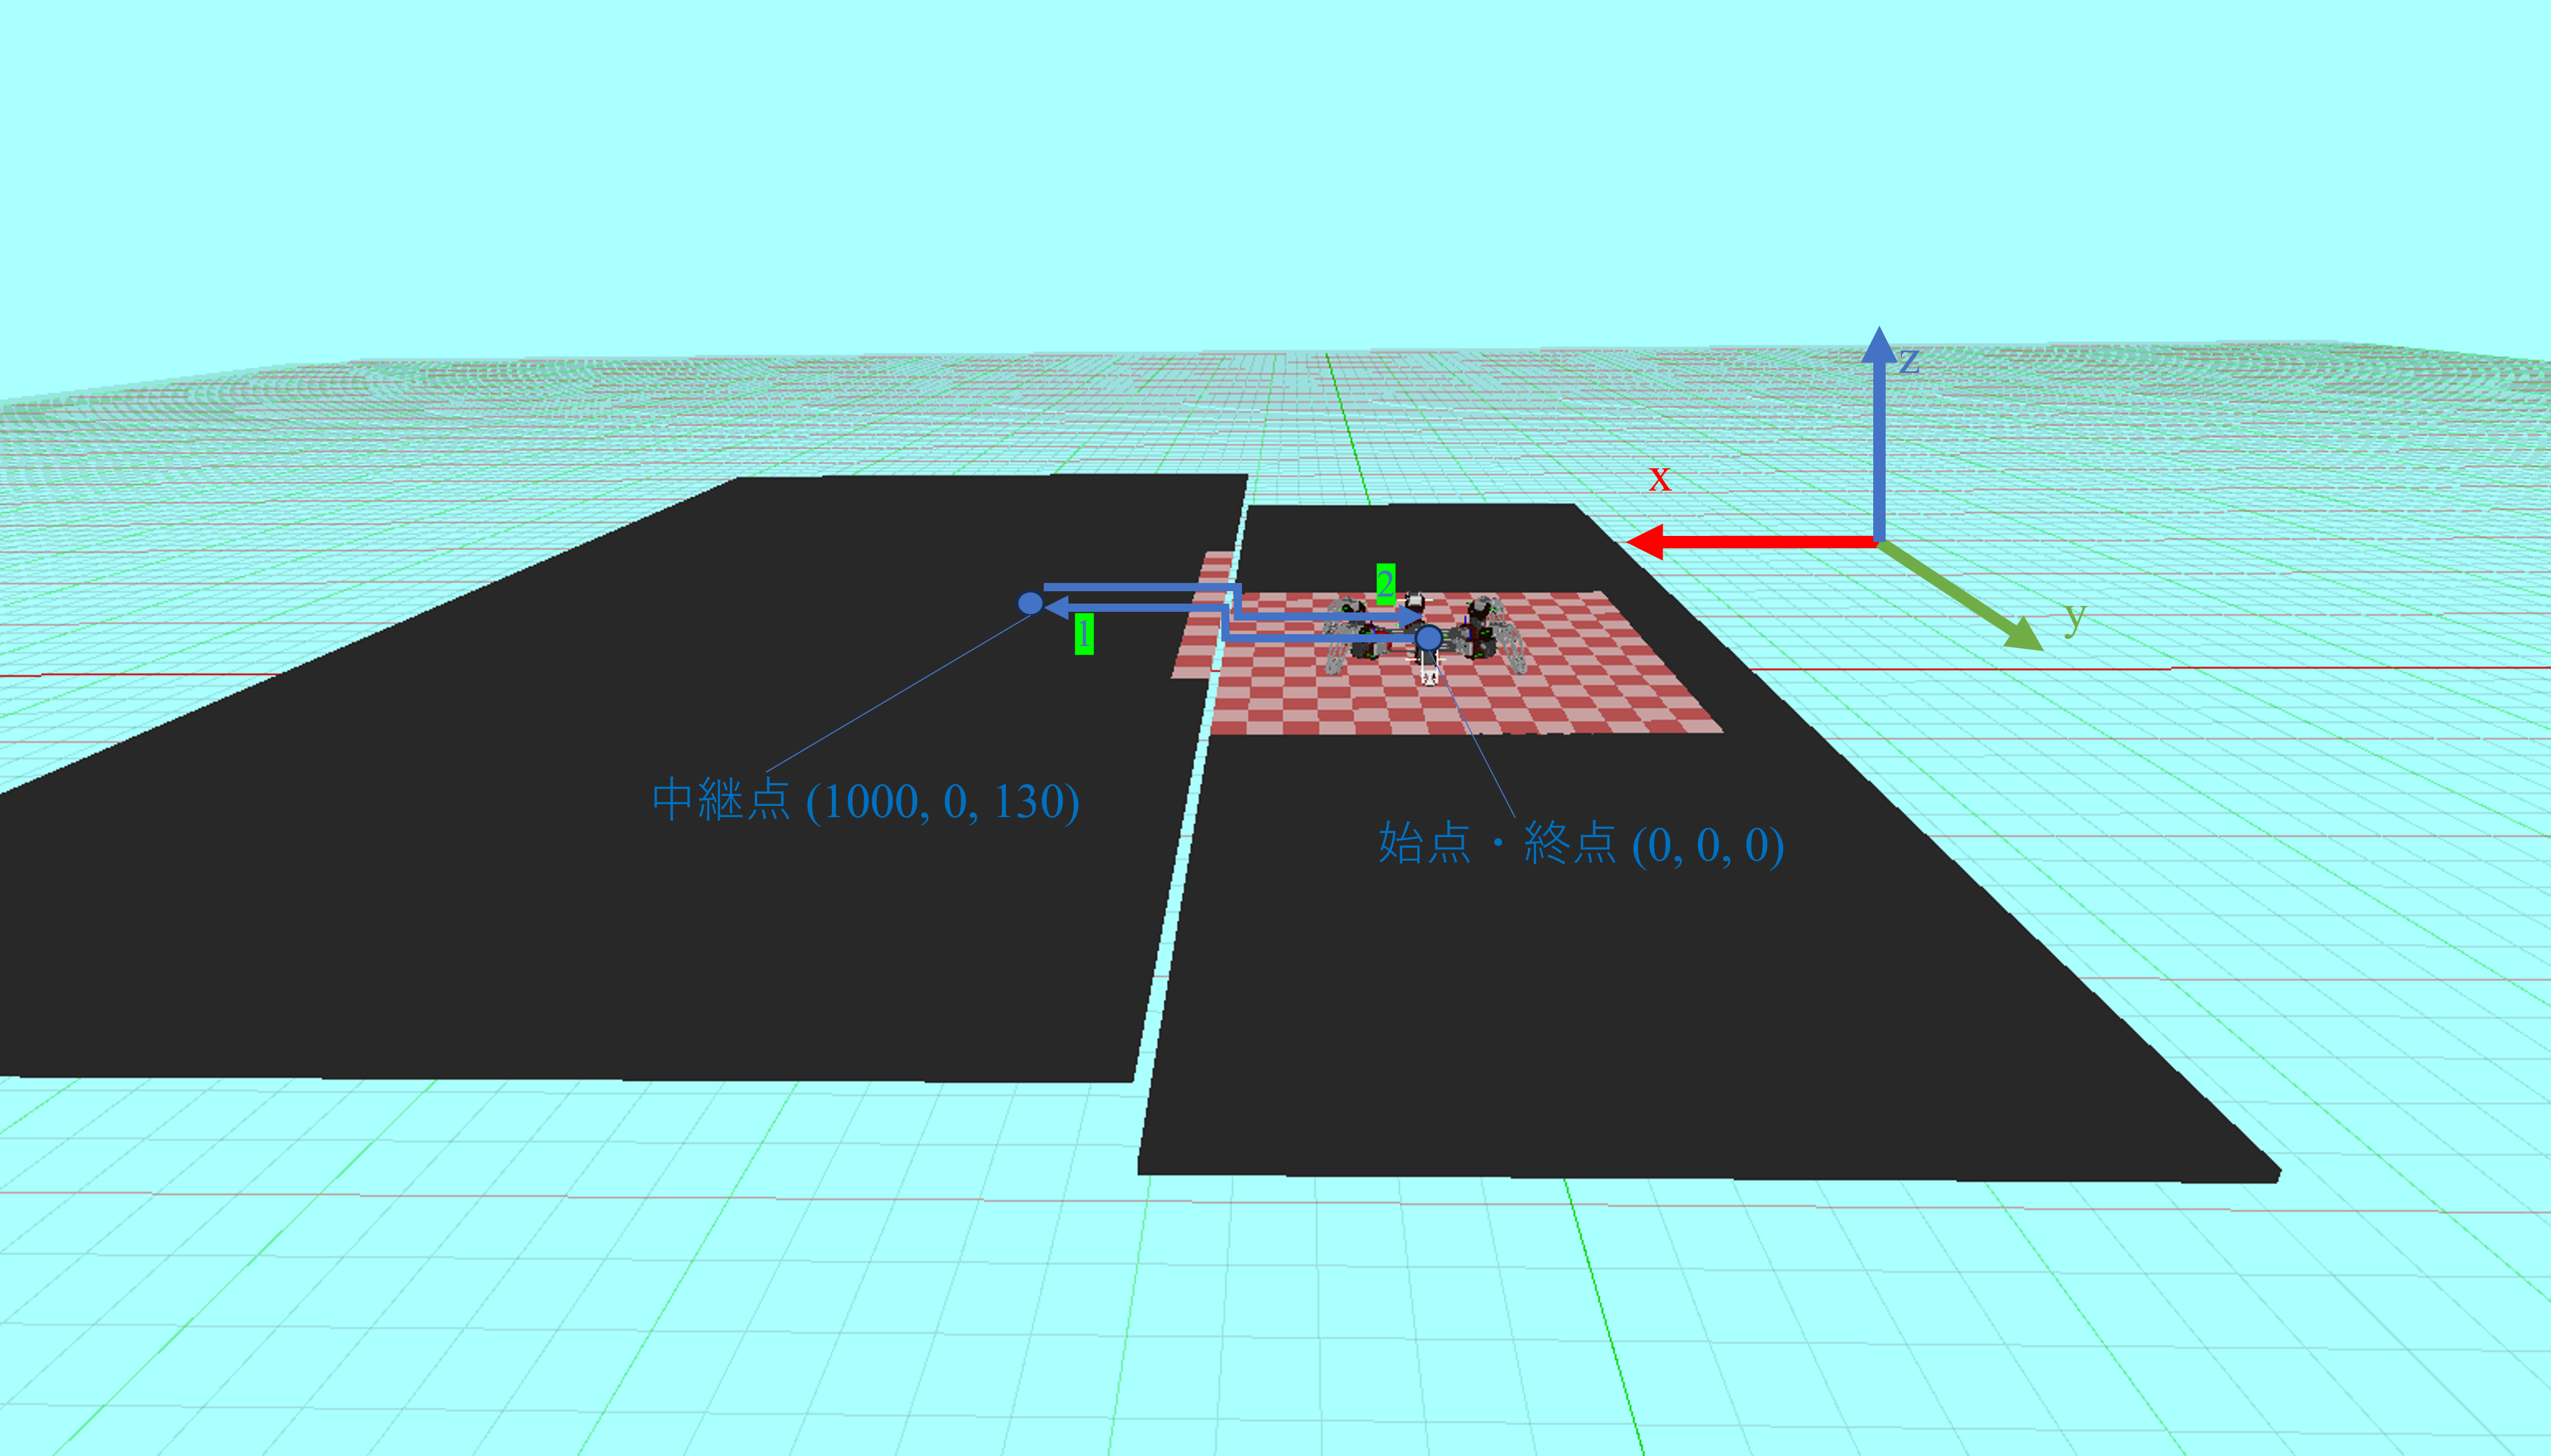
\includegraphics[width=0.7\linewidth,trim={50 50 50 50}, clip]{figure/chapter4/integration_130mm_map.png}
    \caption{Route of Movement on 130mm Steps Terrain}
    \label{fig:ch4_integration_130mm_map}  % chktex 24
  \end{center}
\end{figure}

% chapter4/integration_15deg_map.png
\begin{figure}[htbp]
  \begin{center}
    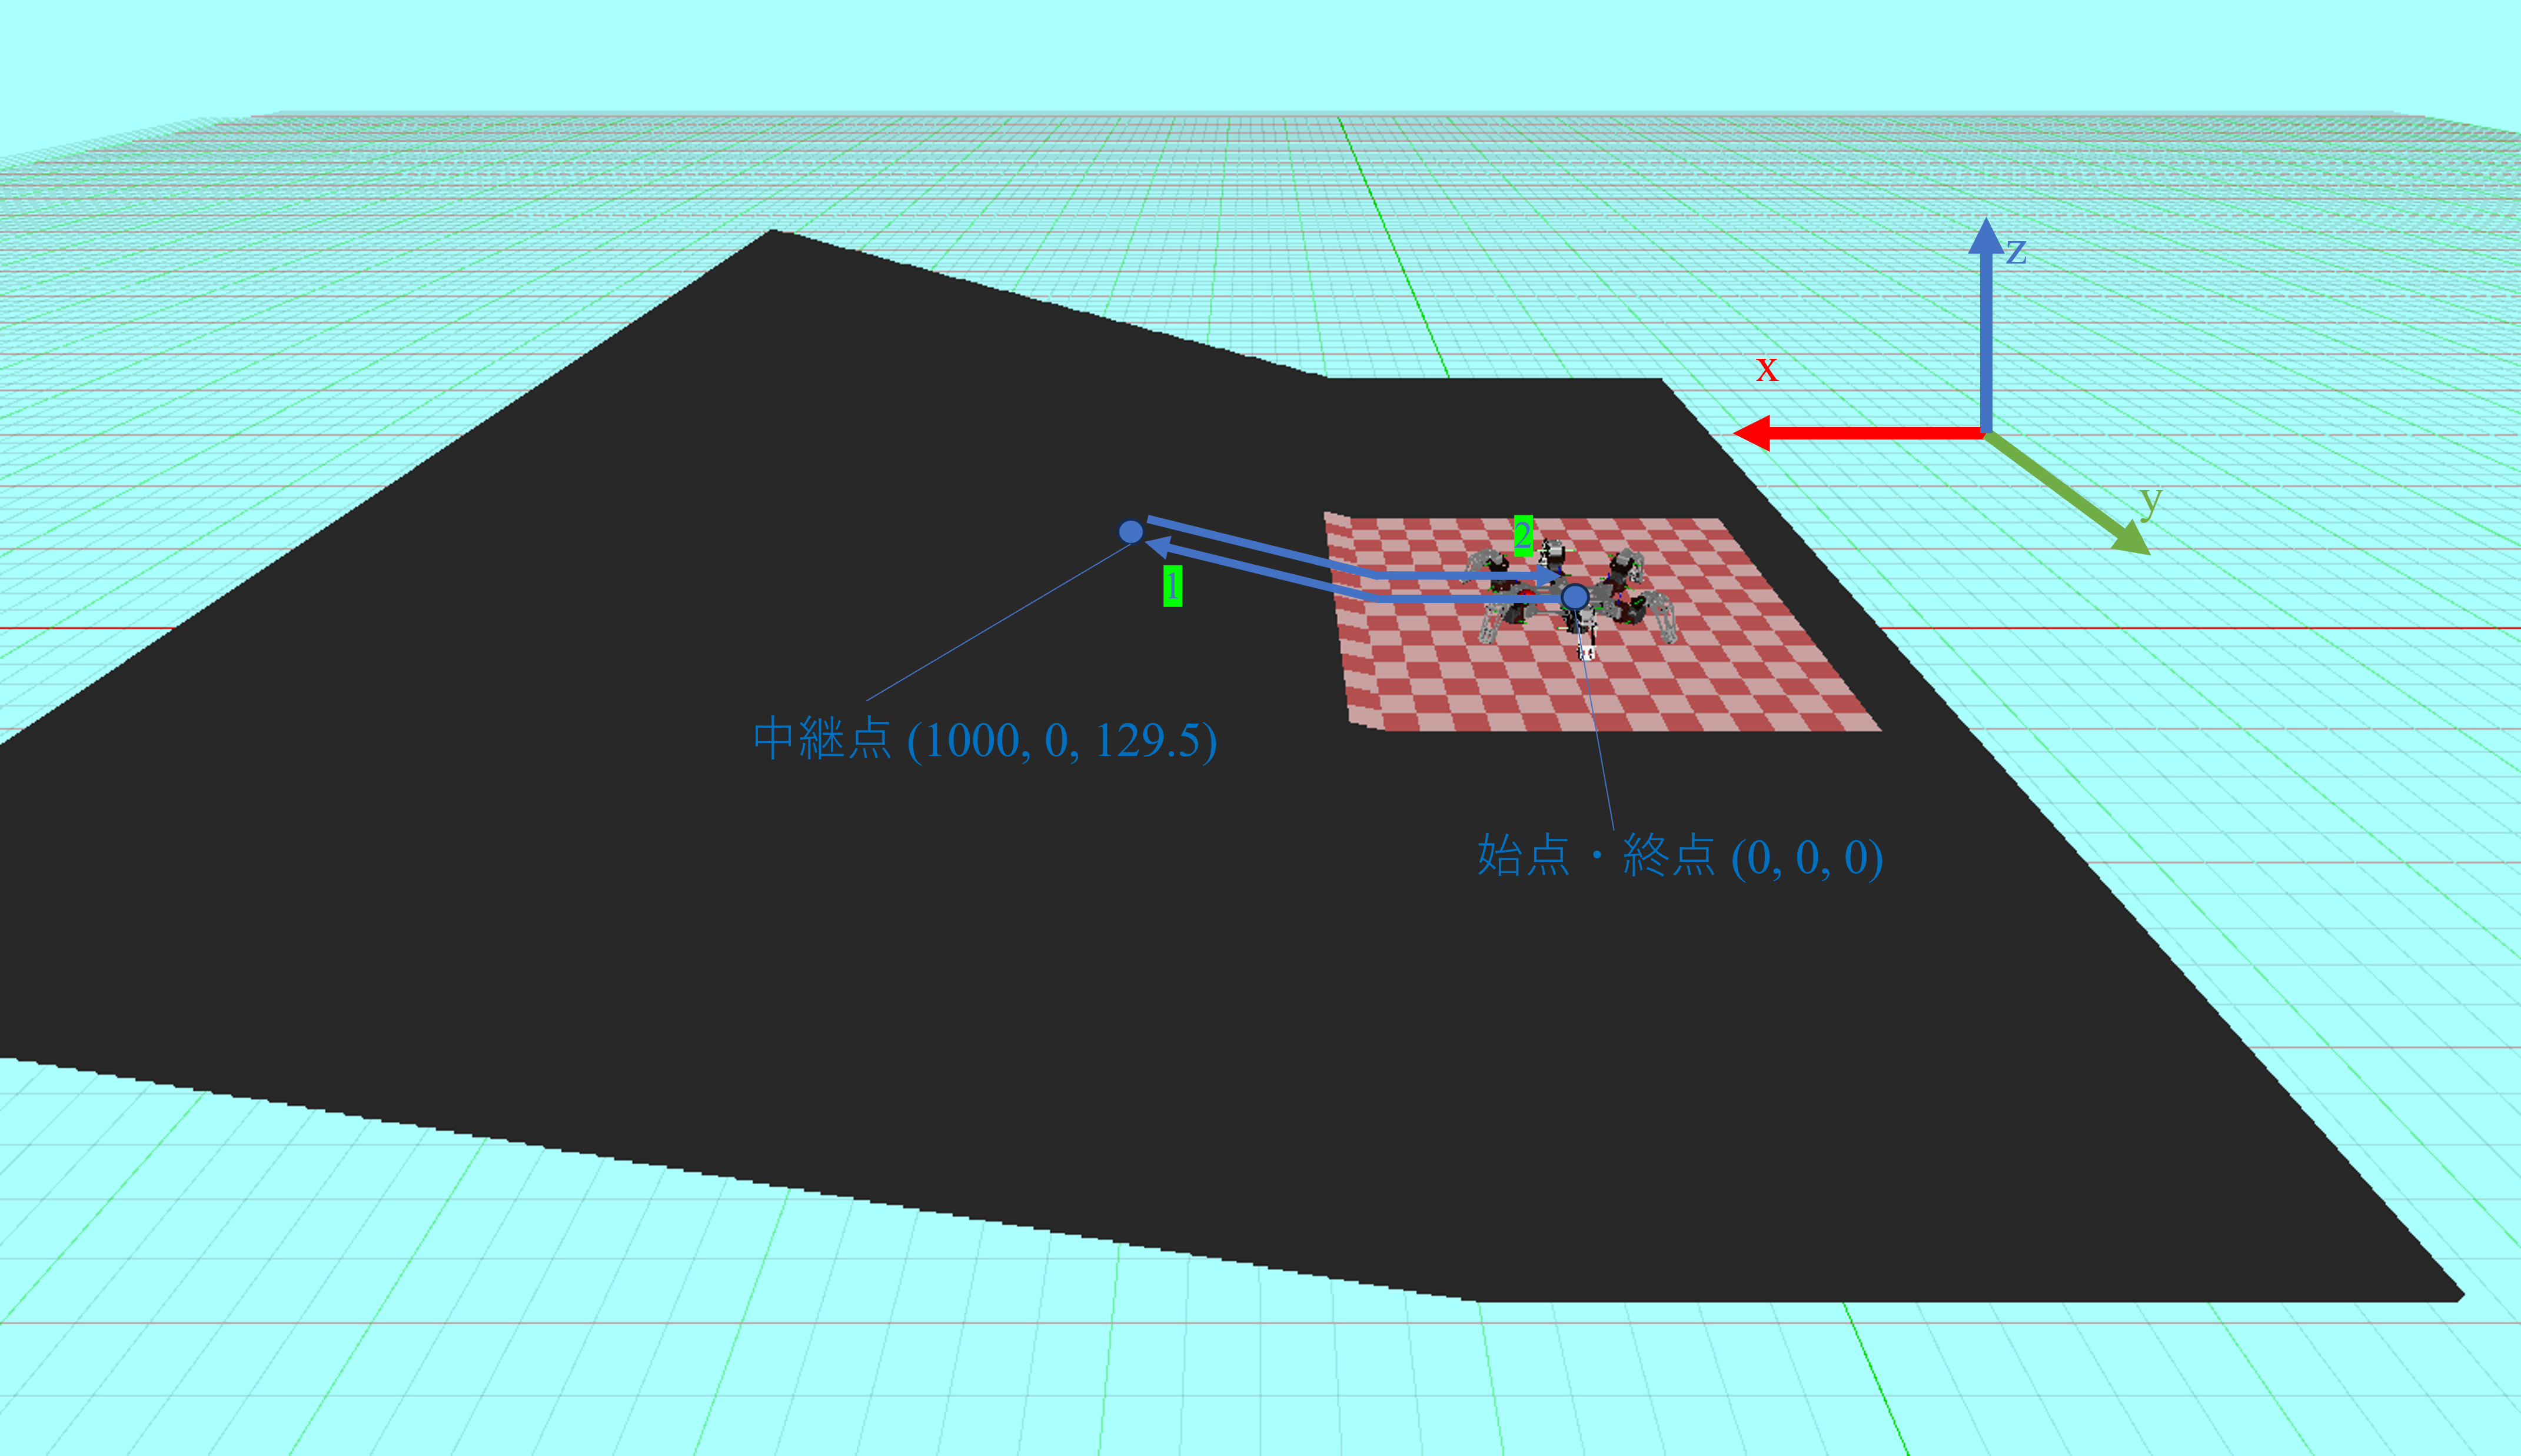
\includegraphics[width=0.7\linewidth,trim={50 50 50 50}, clip]{figure/chapter4/integration_15deg_map.png}
    \caption{Route of Movement on $15^{\circ}$ Slope Terrain}
    \label{fig:ch4_integration_15deg_map}  % chktex 24
  \end{center}
\end{figure}

\subsubsection{シミュレーションの手順}
シミュレーション実験は以下の手順で行う.

\begin{enumerate}
  \item ロボットを始点に配置する.
  \item グラフ探索による自由歩容パターン生成手法を統合したプログラムを用いて,
        経路を追従するような歩容パターンを生成し,歩行させる.
  \item 中継点付近で旋回動作と直進動作を切り替えて歩行することができるかを確認する.
  また歩容パターン生成に失敗することや脚軌道生成に失敗することなく歩行できるかを確認する.
  \item 地形を変更し,(1)から(3)を繰り返す.
\end{enumerate}


\subsection{シミュレーション実験の結果}
\figref{fig:ch4_result_integration}に各地形でのロボットの脚先座標を示す.
\figref{fig:ch4_result_integration}では\figref{fig:ch5_result_turn1},\figref{fig:ch5_result_turn2}と同様に,
軸を取っており,脚先座標も支持脚時を青い丸点,遊脚時を赤い丸点,脚軌道生成に失敗した際の脚軌道の中継点を水色の$\times$で示している.
この図より,脚軌道が可動範囲外を通ることはなかったことがわかる.

また,\figref{fig:ch4_result_integration_graph}に各地形でのロボットの重心の移動軌跡を示す.
\figref{fig:ch4_result_integration_graph}では,横軸をワールド座標系におけるy軸,縦軸をx軸としており,単位は$[mm]$である.
始点から中継点へ移動する際の重心の移動軌跡を赤い線で示し,中継点から終点へ移動する際の重心の移動軌跡を青い線で示しており,
中継点は緑の点で示している.
この図より,ロボットは中継点,終点から最大で100mm程度ずれた位置に到達していることがわかる.


そして,ロボットが歩行する様子を\figref{fig:ch4_result_integration_view_flat},\figref{fig:ch4_result_integration_view_130mm}に示す.
これら図ではロボットの重心の移動軌跡を黄色い線で示している.
加えてロボットの正面をわかりやすくするために,ロボット胴体の正面に赤い球を表示している.
それぞれ,動作の様子をタイムラプス的に撮影した20枚の写真で示している.
右上に01から20までの番号が振られており,00が始点にロボットが配置された状態である.
これらの図よりロボットが直進動作と旋回動作の動作を切り替えていることがわかる.

\newpage

% 脚先を示すグラフ
\begin{figure}[htbp]
  \begin{tabular}{cc}
    \begin{minipage}[t]{0.45\hsize}
      \begin{center}
      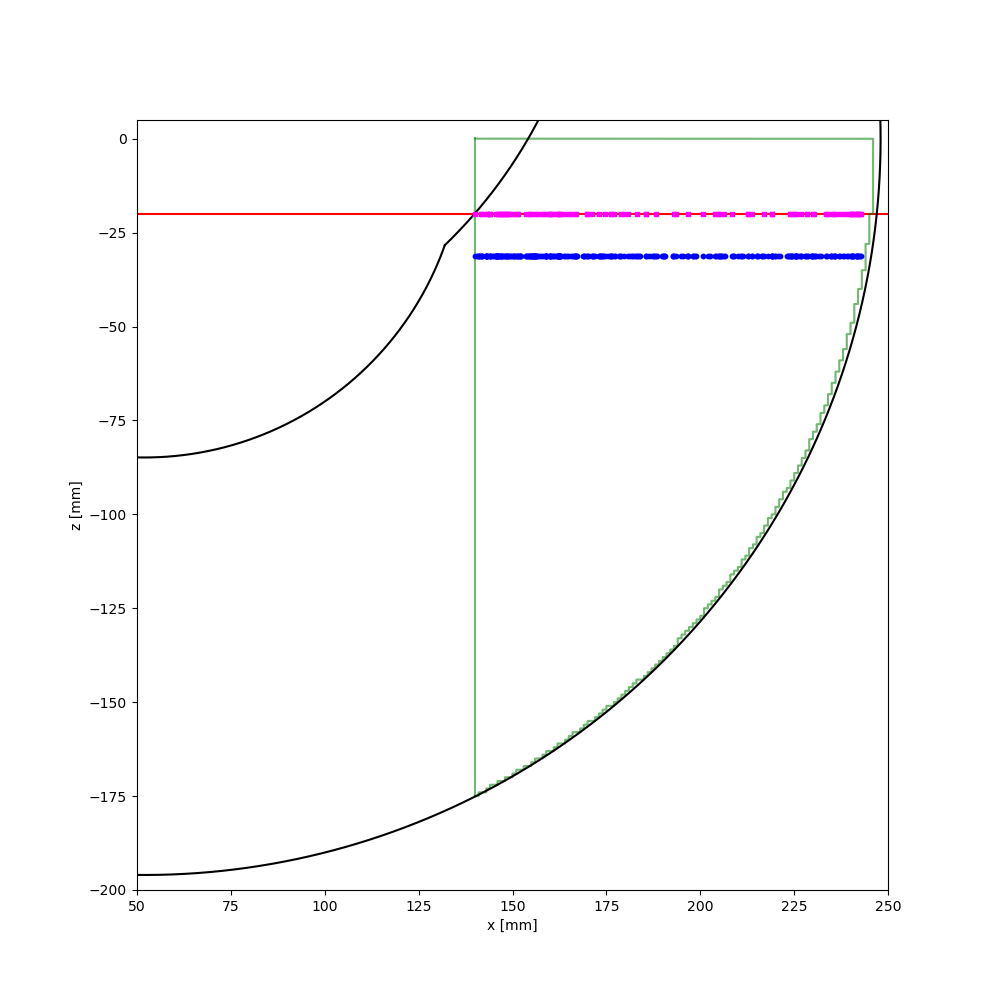
\includegraphics[width=1.0\linewidth,trim={30 30 30 30}, clip]{figure/chapter4/integration/flat.png}
      \text{(a) flat}
      \end{center}
    \end{minipage} 
    &
    \begin{minipage}[t]{0.45\hsize}
      \begin{center}
      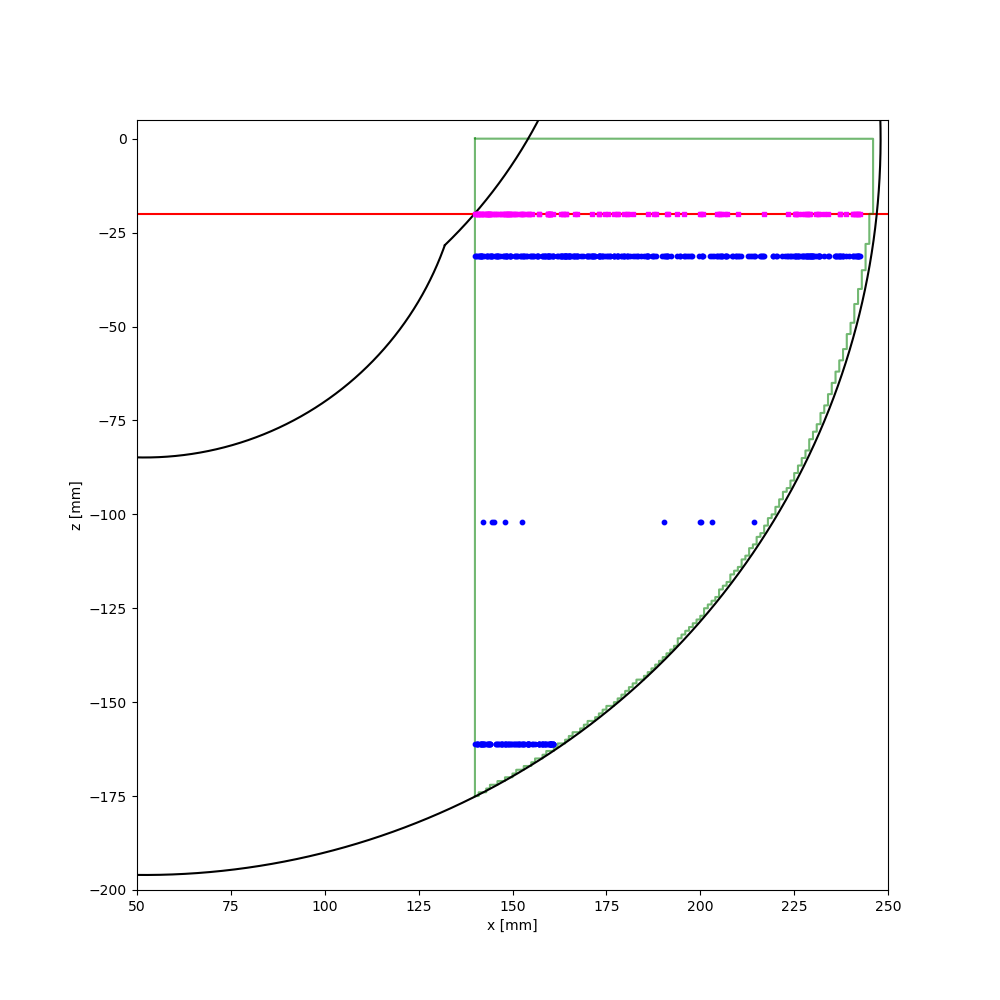
\includegraphics[width=1.0\linewidth,trim={30 30 30 30}, clip]{figure/chapter4/integration/130mm.png}
      \text{(b) 130mm steps}
      \end{center}  
    \end{minipage}
    \\
    \begin{minipage}[t]{0.45\hsize}
      \centering
      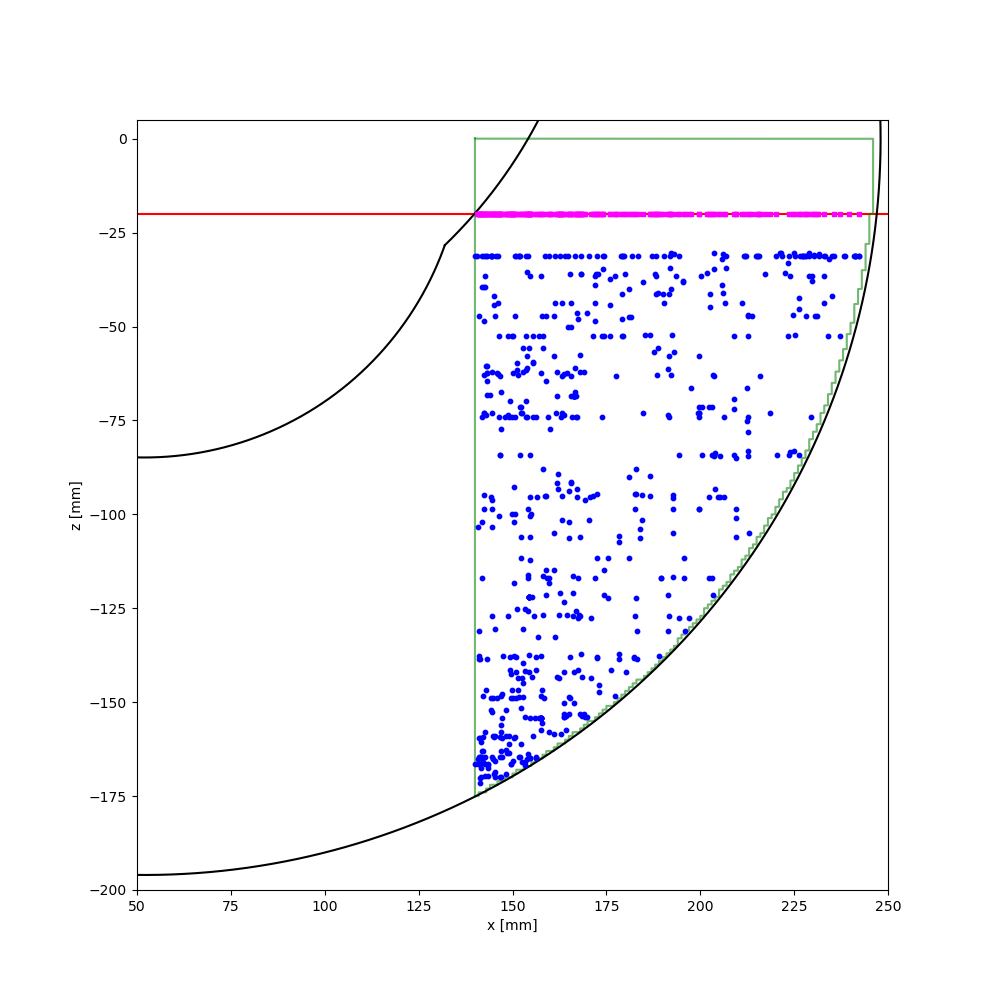
\includegraphics[width=1.0\linewidth,trim={30 30 30 30}, clip]{figure/chapter4/integration/15deg.png}
      \centering
      \text{(c) $15^{\circ}$ slope}
    \end{minipage} 
    &    
    \\
  \end{tabular}
  \caption{Leg Ground Points for Each Terrain}
  \label{fig:ch4_result_integration} % chktex 24
\end{figure}

\begin{figure}[htbp]
  \begin{tabular}{ccc}
    \begin{minipage}[t]{0.3\hsize}
      \begin{center}
      \fbox{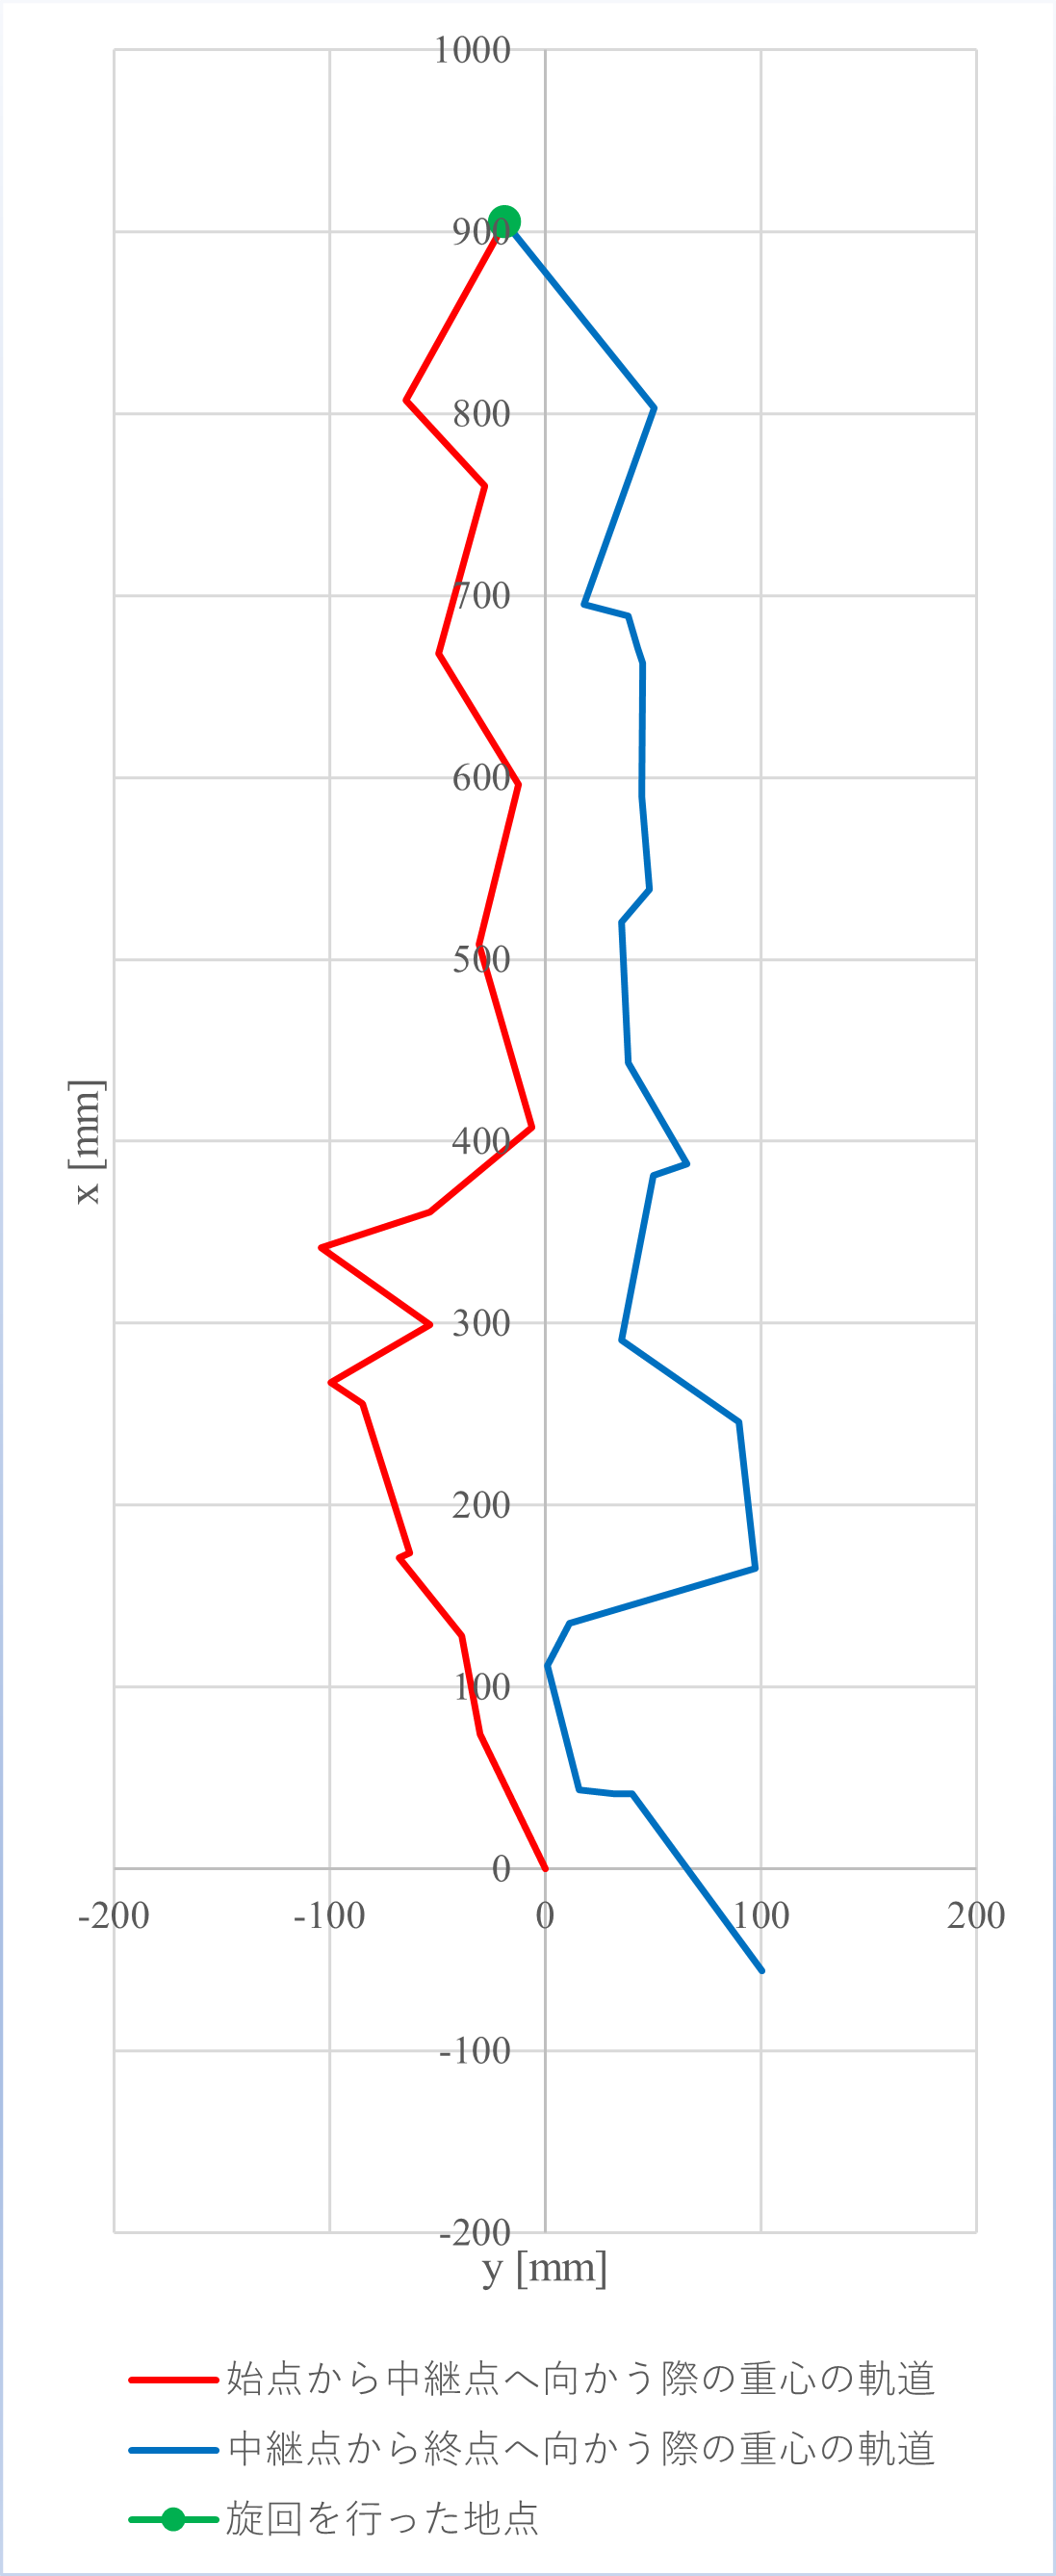
\includegraphics[width=0.9\linewidth]{figure/chapter4/integration/flat_com.png}}
      \text{(a) flat}
      \end{center}
    \end{minipage} 
    &
    \begin{minipage}[t]{0.3\hsize}
      \begin{center}
      \fbox{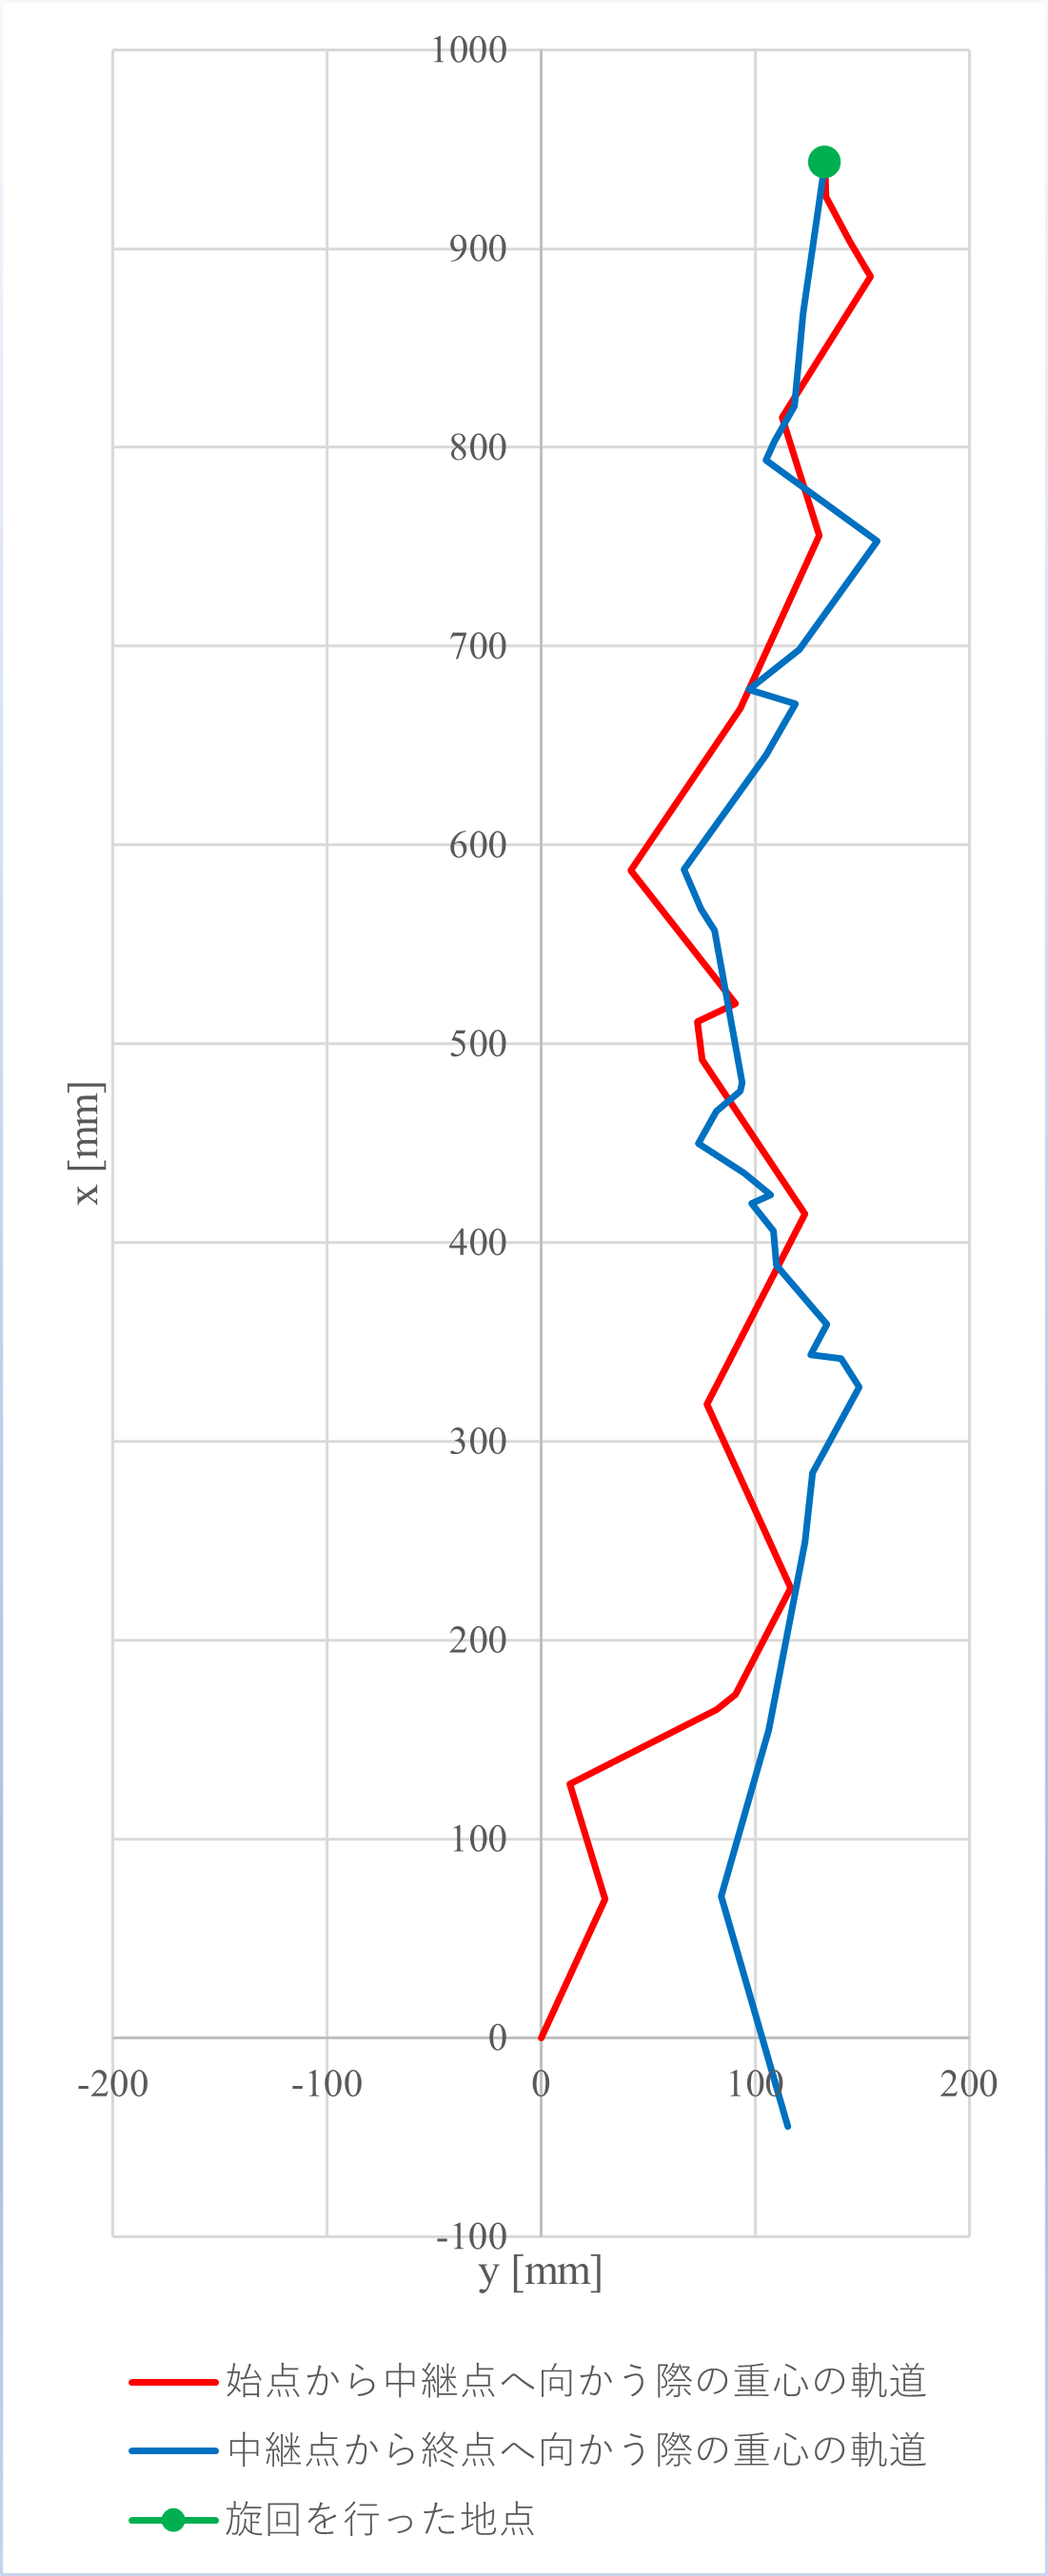
\includegraphics[width=0.9\linewidth]{figure/chapter4/integration/130mm_com.png}}
      \text{(b) 130mm steps}
      \end{center}  
    \end{minipage}
    &
    \begin{minipage}[t]{0.3\hsize}
      \centering
      \fbox{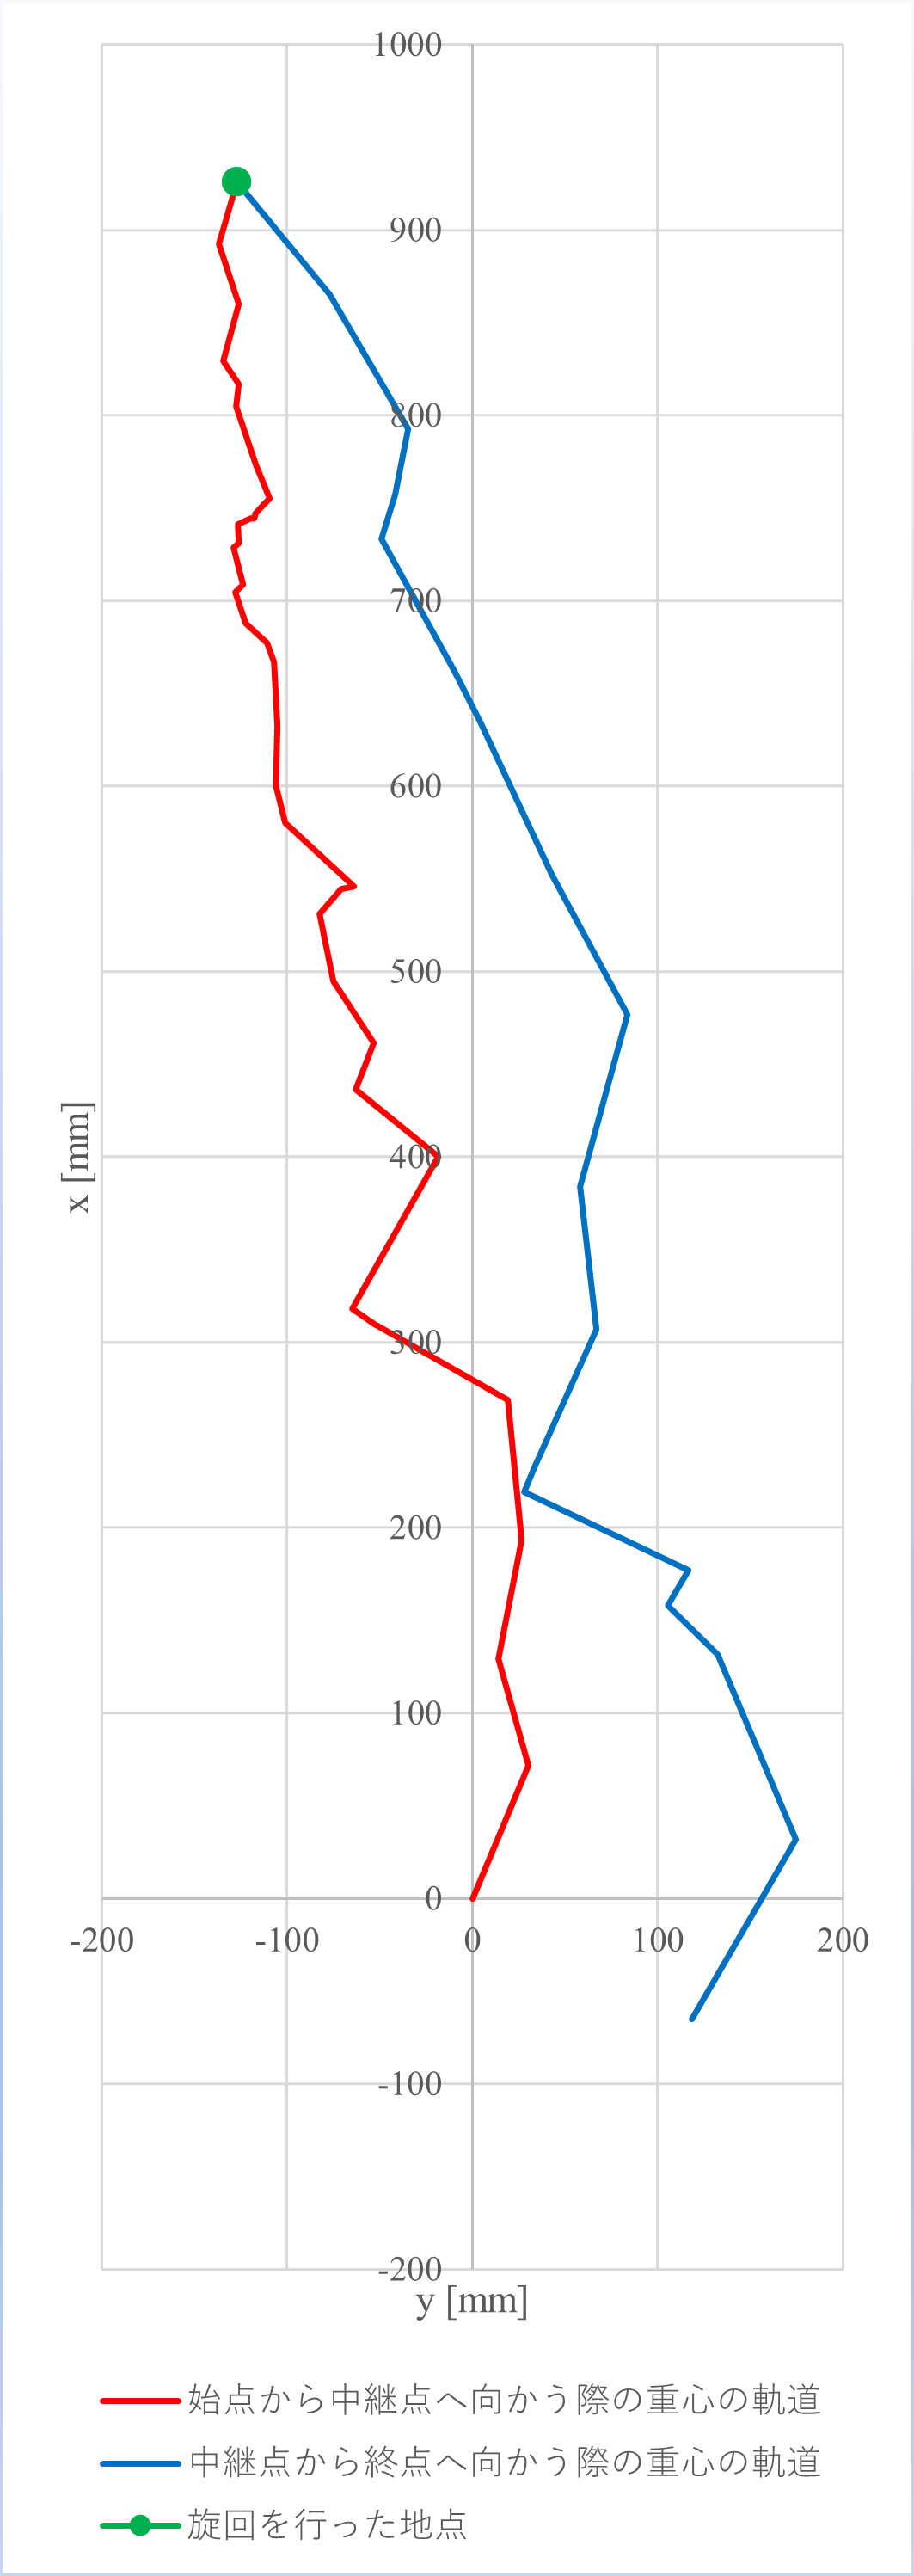
\includegraphics[width=0.9\linewidth]{figure/chapter4/integration/15deg_com.png}}
      \centering
      \text{(c) $15^{\circ}$ slope}
    \end{minipage}  
    \\
  \end{tabular}
  \caption{Path of Center of Mass for Each Terrain}
  \label{fig:ch4_result_integration_graph} % chktex 24
\end{figure}

\begin{figure}[htbp]
  \begin{center}
    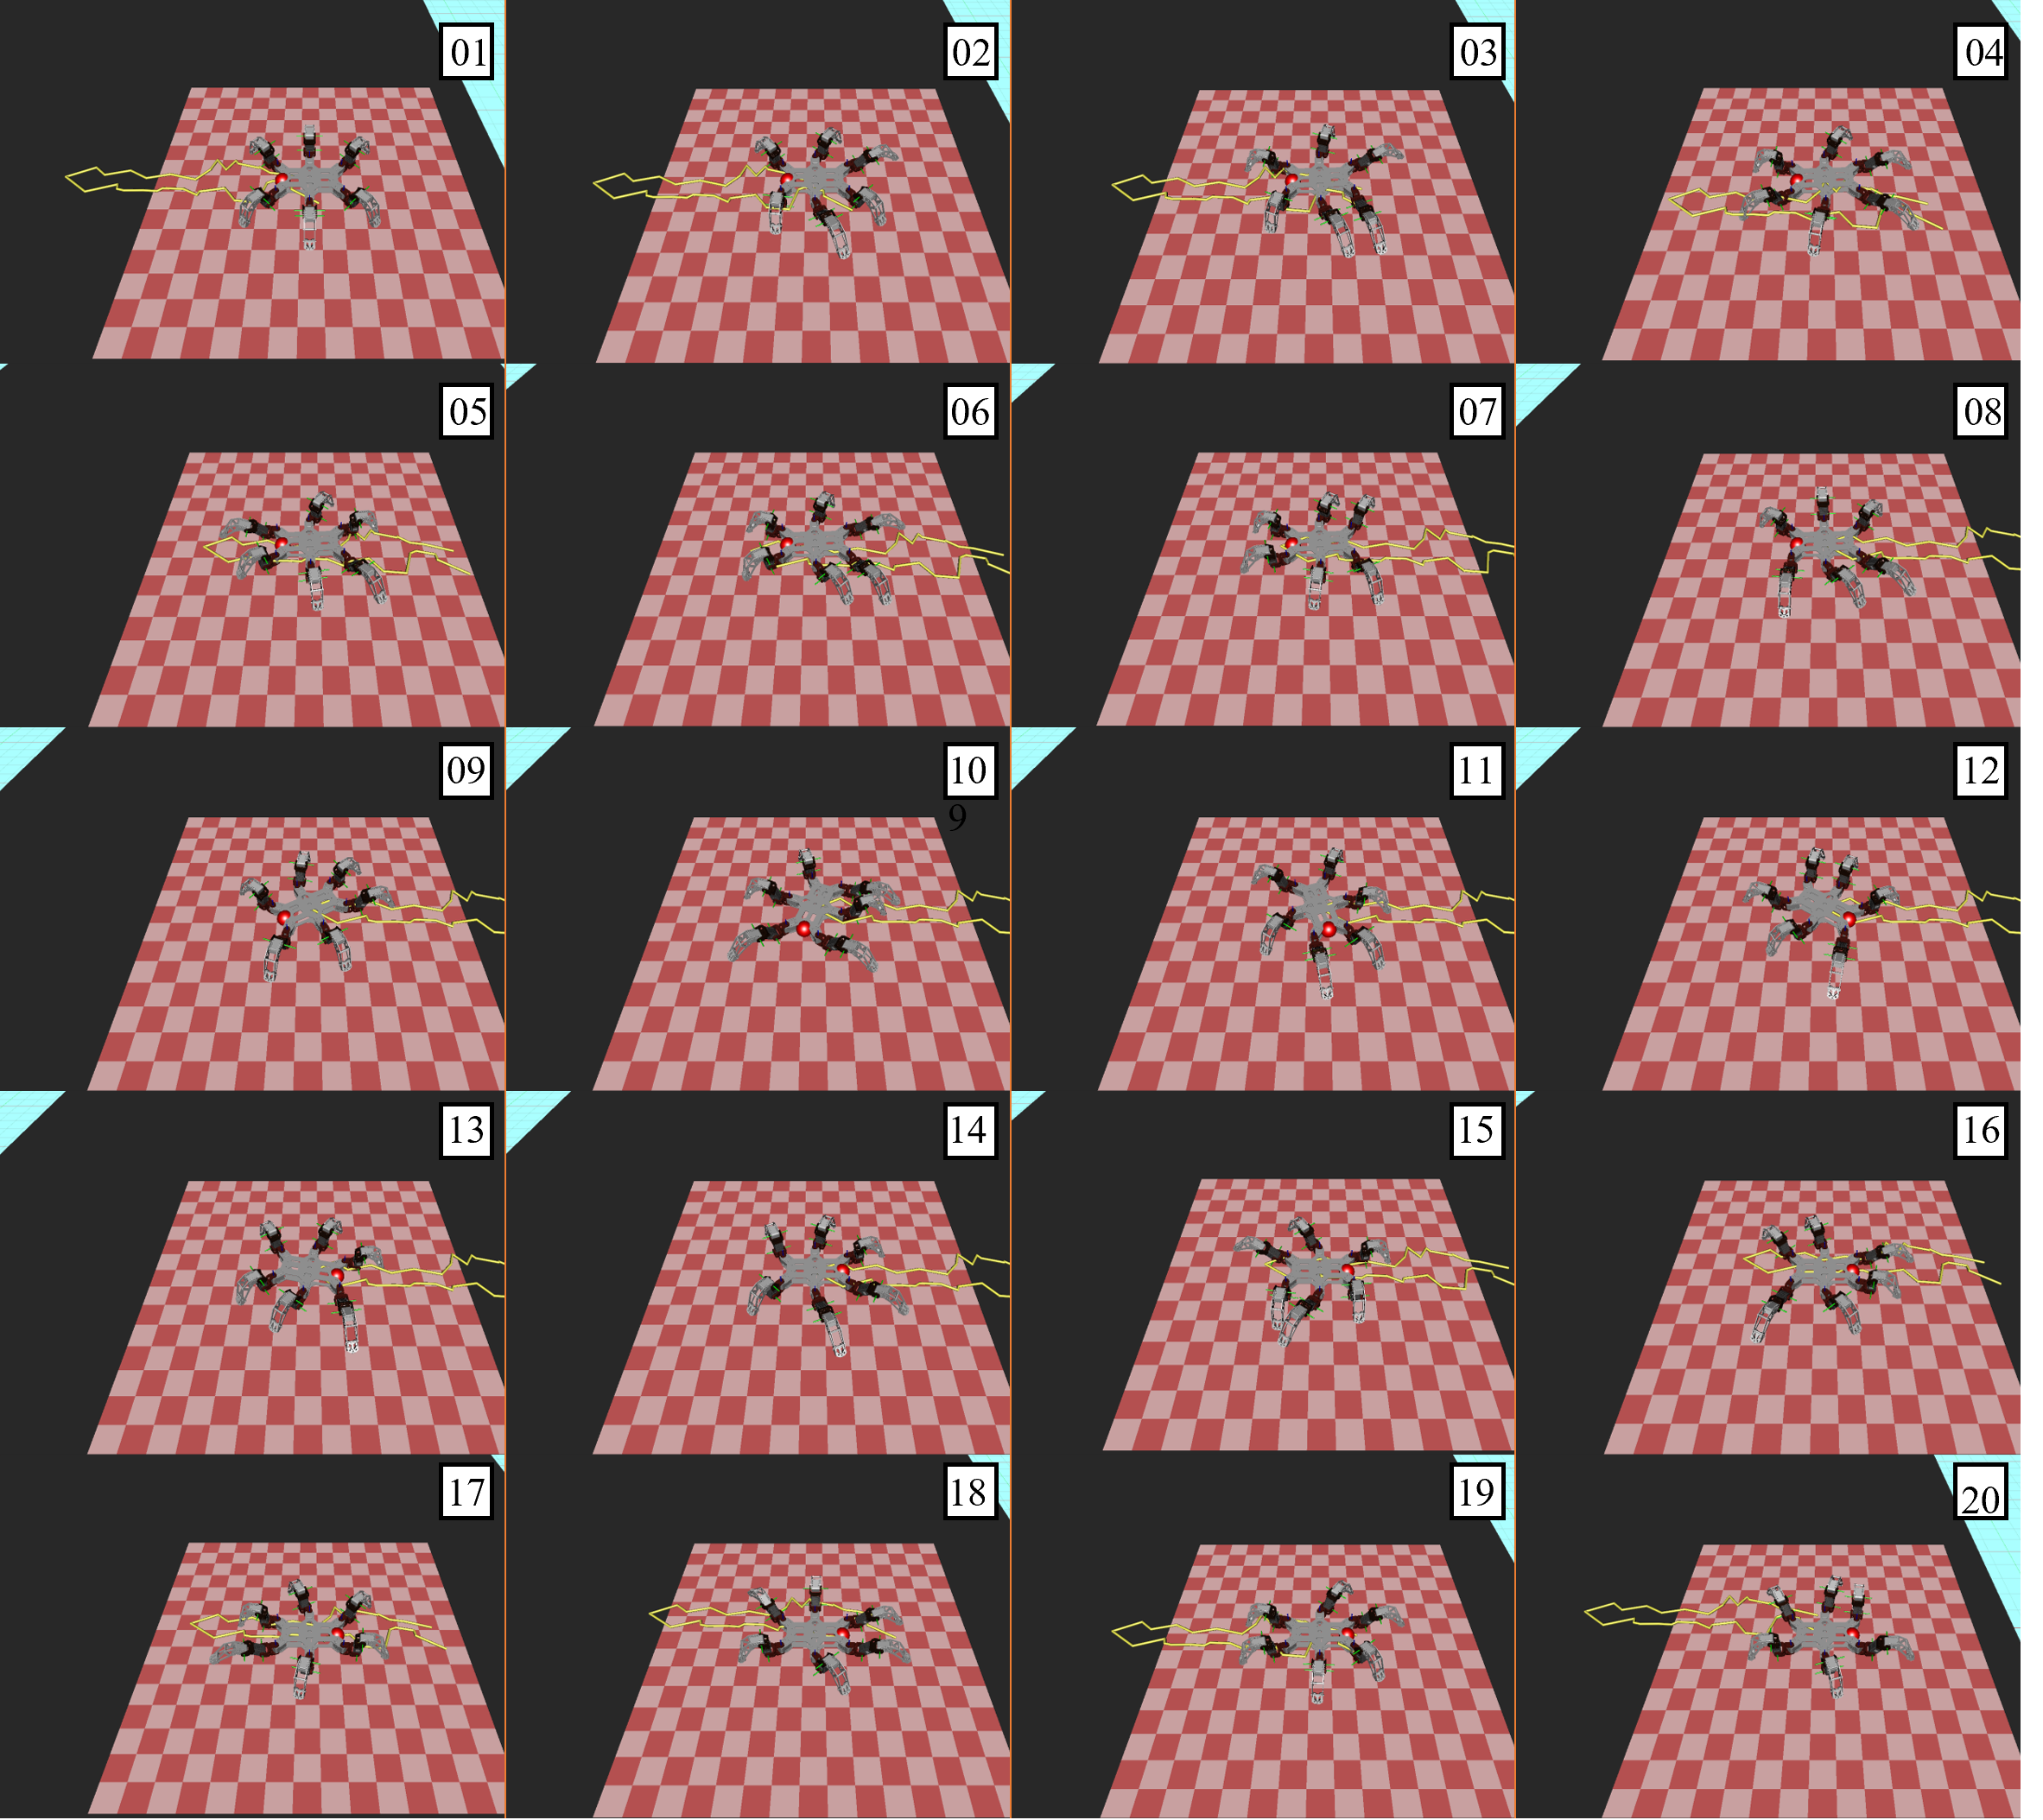
\includegraphics[width=1.0\linewidth]{figure/chapter4/integration/flat_view.png}
    \caption{View of Operation on a Flat}
    \label{fig:ch4_result_integration_view_flat}  % chktex 24
  \end{center}
\end{figure}

\begin{figure}[htbp]
  \begin{center}
    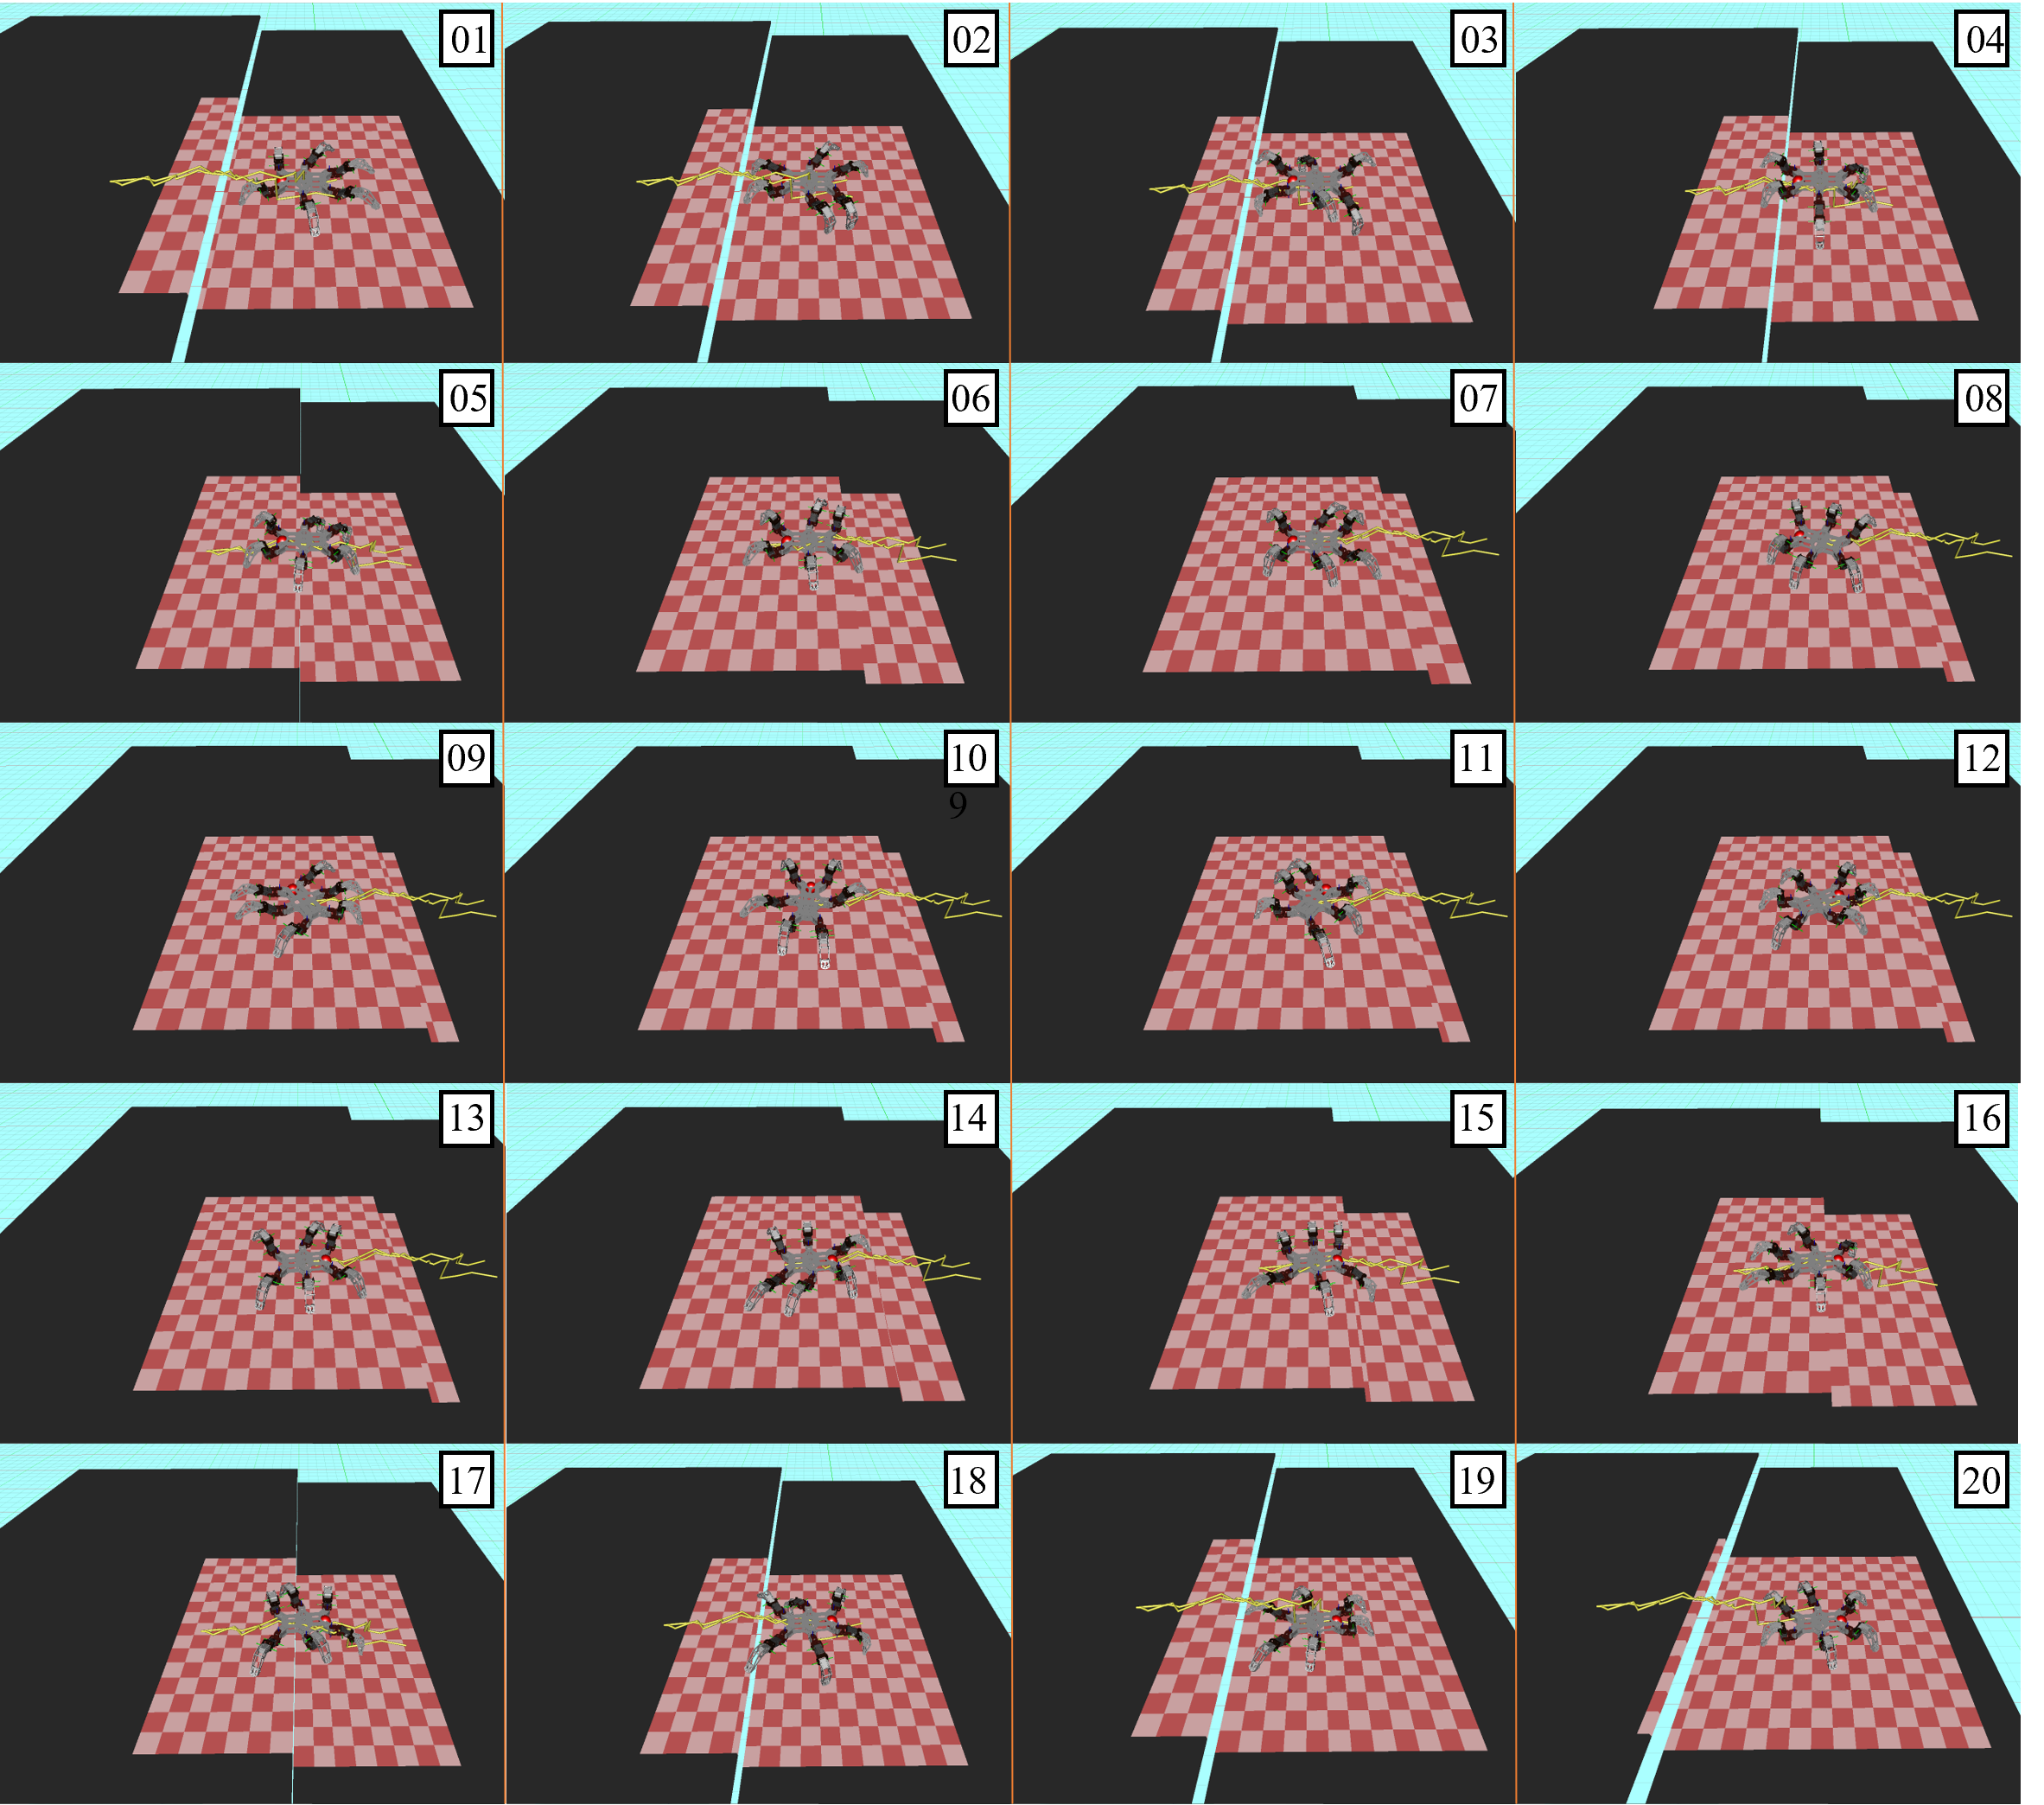
\includegraphics[width=1.0\linewidth]{figure/chapter4/integration/130mm_view.png}
    \caption{View of Operation on a 130mm Step}
    \label{fig:ch4_result_integration_view_130mm}  % chktex 24
  \end{center}
\end{figure}

\begin{figure}[htbp]
  \begin{center}
    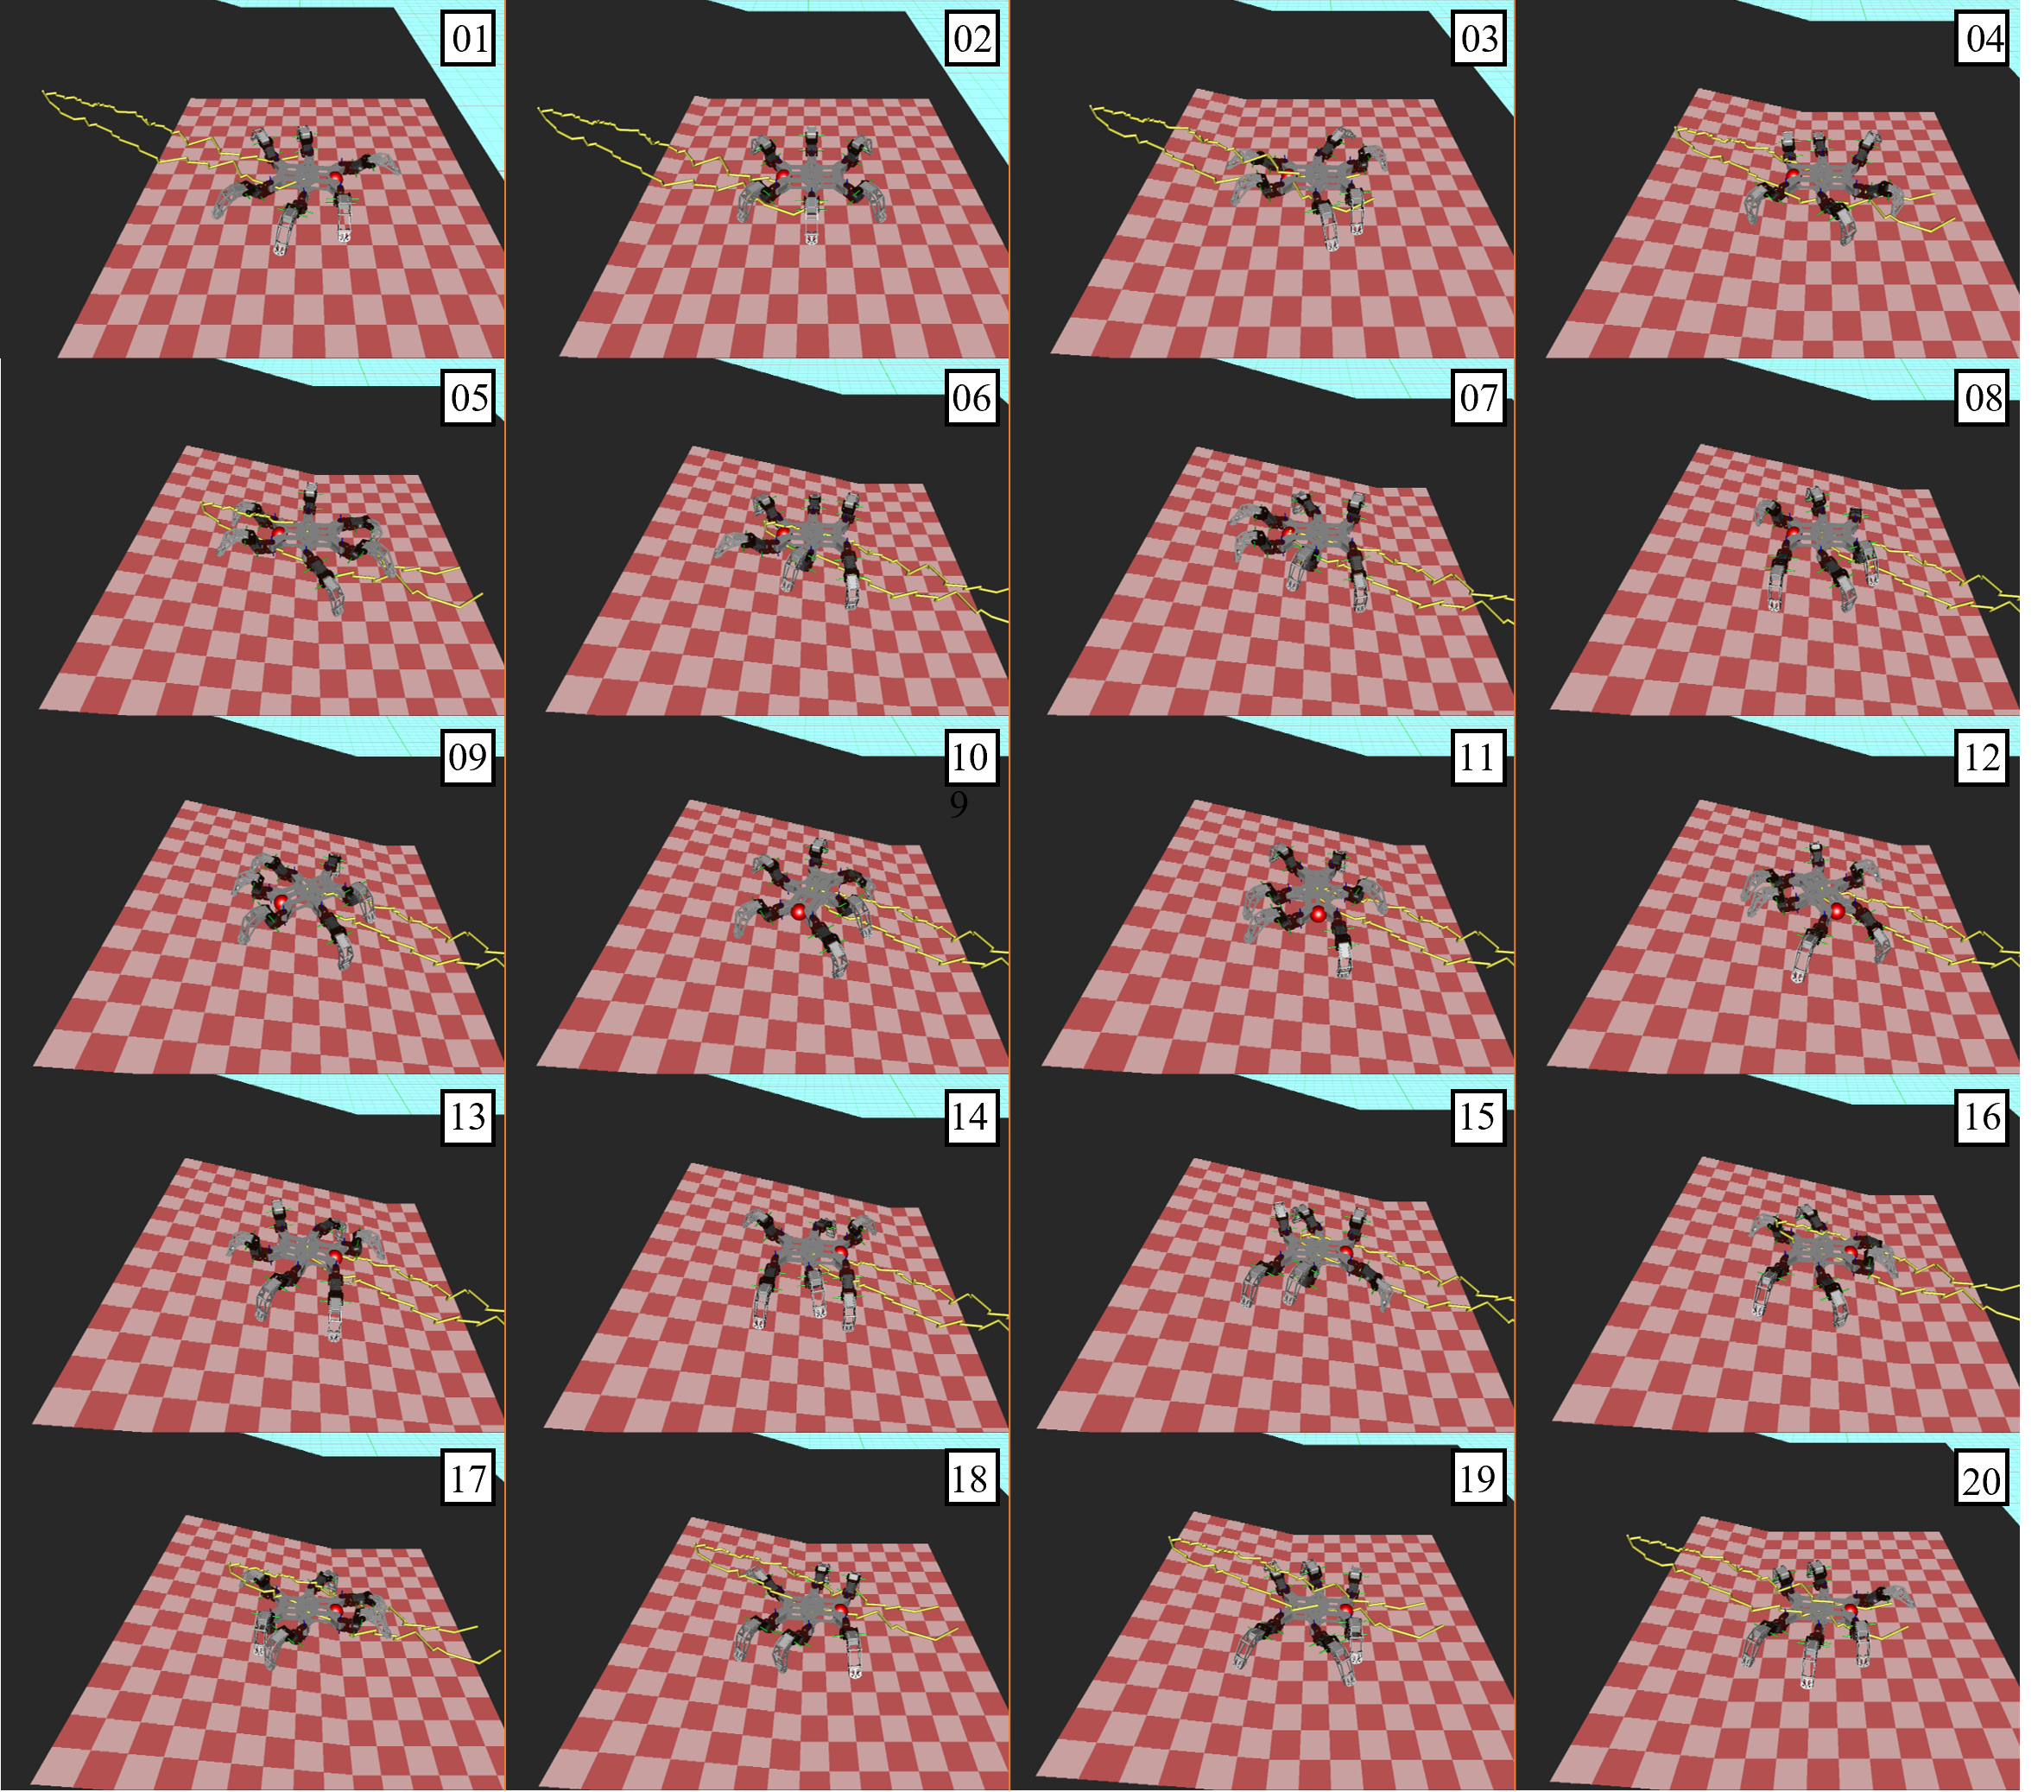
\includegraphics[width=1.0\linewidth]{figure/chapter4/integration/15deg_view.png}
    \caption{View of Operation on a $15^{\circ}$ Slope}
    \label{fig:ch4_result_integration_view_15deg}  % chktex 24
  \end{center}
\end{figure}

\subsection{考察}
結果よりロボットは直進動作と旋回動作を切り替えて歩行することができたため,
実装した自由歩容パターンを統合したプログラムによって,
直進動作と旋回動作を組み合わせた歩容パターンを生成することができるといえる.

また\figref{fig:ch4_result_integration}より,脚軌道生成に失敗することなく歩行することができたため,
最小半径を140mmに設定することが脚軌道生成の失敗を防ぐために有効であるといえる.

\figref{fig:ch4_result_integration_graph}より,
ロボットは指定した通りに動作を切り替えることができたが,
指定した経路を追従できなかったことがわかる.
これは,グラフ探索の評価関数において,
重心をもっとも大きく移動するノードが高く評価されることにより,
指定された地点から離れてしまったとしても,
重心をもっとも大きく移動するノードを選択してしまうためであると考えられる.
本研究では,脚軌道生成の失敗を防ぐことを目的としているため,
経路の追従については考慮していなかったが,
実際にロボットに作業をさせる際には,経路の追従も考慮する必要があるといえるだろう.
経路を適切に追従させるためには,評価関数を変更することが考えられる.
評価関数において,中継点への到達を重視することで,
経路を追従するような歩容パターンを生成することができると考えられる.
